\documentclass[conference]{IEEEtran}
%\IEEEoverridecommandlockouts
% The preceding line is only needed to identify funding in the first footnote. If that is unneeded, please comment it out.
\usepackage{cite}
\usepackage{amsmath,amssymb,amsfonts,mathtools}
\usepackage{algorithmic}
\usepackage{graphicx}
\usepackage{textcomp}
\usepackage{xcolor}
%\usepackage[numbers,sort&compress]{natbib}
%\usepackage{hyperref}

\def\BibTeX{{\rm B\kern-.05em{\sc i\kern-.025em b}\kern-.08em
    T\kern-.1667em\lower.7ex\hbox{E}\kern-.125emX}}
\renewcommand{\IEEEQED}{\IEEEQEDopen}

\newtheorem{theorem}{Theorem}
\newtheorem{lemma}{Lemma}
\newtheorem{proposition}{Proposition}
\newtheorem{corollary}{Corollary}
\newtheorem{remark}{Remark}
\begin{document}

\title{The Influence of Canyon Shadowing on Device-to-Device
  Connectivity in Urban Scenario
%  on Poisson-Voronoi Street Systems
%\thanks{Identify applicable funding agency here. If none, delete this.}
}

\author{\IEEEauthorblockN{Quentin Le Gall\IEEEauthorrefmark{1}, Bart\l{}omiej B\l{}aszczyszyn\IEEEauthorrefmark{2}, Elie Cali\IEEEauthorrefmark{1} and Taoufik En-Najjary\IEEEauthorrefmark{1}}
\IEEEauthorblockA{\IEEEauthorrefmark{1}Modelling and Statistical Analysis, Orange Labs Networks, Ch\^{a}tillon, France\\
Email: quentin1.legall@orange.com, elie.cali@orange.com and taoufik.ennajjary@orange.com}
\IEEEauthorblockA{\IEEEauthorrefmark{2}Inria-ENS, Paris, France\\
Email: bartek.blaszczyszyn@ens.fr}}

\maketitle

\begin{abstract}
Using percolation theory, we study the  feasibility  of large-scale  connectivity  of  relay-augmented D2D  networks  in urban scenario featuring haphazard system of streets and  canyon shadowing allowing only for line-of-sight (LOS) communications in a limited  finite range.
We use a homogeneous  Poisson-Voronoi  tessellation (PVT) model of streets with   homogeneous Poisson users (devices)  on its edges 
and independent Bernoulli relays on the vertices. 
As customary in percolation approach, good connectivity the notwork   is  indicated by the positive probability of the  existence of an infinite connected component of the respective graph of connections. Finding and estimating by simulation appropriate critical values of the  model parameters we observe that: Canyon shadowing requires usage of relays, with our model predicting at  least 71.3\%  of  crossroads  equipped with them.  If the mean street length 
is not larger than  some threshold (predicted to 0.743 of the communication range; which might be  the case in a typical urban scenario) then small density  of  users  can  be  compensated by equipping more  crossroads  with relays.
%the required  proportion increases from 71.3\%  to 1 when the mean street length %goes  from~0 to 0.743  of the D2D connectivity radius.
If the mean street length exceeds this latter threshold,
good connectivity requires some minimal density of users compensated by the relays
in a way we make explicit. The existence of the above regimes bring interesting qualitative  arguments to the discussion on the  possible D2D deployment  scenarios
and the quantitative prediction of the  critical  values might be improved
using more adequate models.
\end{abstract}

\begin{IEEEkeywords}
Device-to-device networks, relays, connectivity, shadowing, continuum percolation, simulation
\end{IEEEkeywords}

\section{Introduction}
%\subsection{Motivations}
The fifth generation (5G) of mobile networks currently concentrates an
intensive research effort covering broad fields such as security,
energy consumption, radio communications or resource allocation
\cite{andrews2014will, boccardi2014five,wang2014cellular}. One of the main technical challenges of 5G remains to
face the exponential growth of mobile data traffic while keeping up
with the quality of service (QoS). Device-to-Device (D2D) is deeply
investigated in this regard \cite{tehrani2014device}. Coverage extension could
also be achieved thanks to multihop D2D networks \cite{lin2013comprehensive}. This
opens the way to crowd networking and uberization of telecommunications networks \cite{asadi2014survey}, which represent high economic stakes for operators. 

As a matter of fact, studying the technical feasibility of
large-scale connectivity of D2D networks seems critical for
operators. To this end, resorting to mathematical models amenable to
numerical simulations remains a safe and necessary prelude to massive
investments. Since the seminal paper~\cite{gilbert1961random} of Gilbert, the
question of large-scale connectivity in telecommunication networks has mathematically been dealt with using percolation theory: the network is modelled by an infinite  graph whose edges represent possible connections on the network, called the connectivity graph. Good connectivity of the network is then interpreted as the existence of an infinite connected component of the aforementioned graph with positive probability: this is called percolation \cite{grimmett1999percolation, meester_continuum_1996}. \\
\indent Over the years, mathematical models have been refined so as
to take into account more physical features,
including  interference, shadowing and  various street system models. 
%, etc. cf Section~\ref{ss.RelatedWorks}.
In this paper, we introduce the canyon shadow assumption applied to some 
previously used street system and study its impact on the
connectivity properties of D2D network using percolation theory.

\noindent More precisely, following~\cite{cali2018percolation}, we model the street system via an  homogeneous  Poisson-Voronoi
tessellation (PVT) and  users (equipped with mobile devices) as a
homogeneous Cox process supported by the PVT. Crucial,
dimensionless and scale-invariant parameters of this model are the mean number of users per
typical street of the network,  denoted in what follows by $U$, 
and the mean number of hops necessary to
ensure connectivity on a typical street of the network, denoted
by $H$. Note that $U$ depends on the density of the street system and the density of users,
while $H$ represents the interplay between the street system 
and the transmission range related to D2D technology.

As the main novelty of our work, we consider  the {\em canyon effect
  of shadowing}  allowing  only for  line-of-sight (LOS) connections
on the streets: only network nodes located on
the  same street, and whose relative distance is less than a certain
threshold can establish communication.
%(are connected). 
This assumption, combined
with the PVT-Cox  model of the streets and users, requires the presence of relays located
at crossroads (i.e. vertices of the PVT) in order to achieve the connectivity between adjacent
streets. Indeed, the junction between adjacent streets in our PVT street model are punctual, and the probability of occurrence of a Cox user at a precise point is 0 \cite[Section 5.2]{chiu_stochastic_2013}. Relays can then either be interpreted as physical antennas or as additional users not modelled by the considered Cox process.
We chose to model these relays via a Bernoulli process \cite[Section 2.2]{chiu_stochastic_2013}
on the vertices of the PVT: the relays are placed independently at 
the vertices  of the PVT with a fixed constant probability denoted
by $p$. This probability can also be interpreted as the total proportion of crossroads of the street system equipped with relays. 

Our goal is to show how  the  connectivity properties of the D2D network
depend on  the mean number of users per
typical street $U$, the mean number of hops necessary to
ensure connectivity on a typical street $H$, and the  proportion $p$ of
crossroads equipped with relays. 
To this end, using appropriate simulation techniques,  we study  the  percolation regime of the considered
model. 



%\subsection{Main results}
The main results of this paper are the following ones:

\paragraph{Minimal relay proportion} We proved that there exists a minimal relay proportion $p_c$ below which there
  is no percolation of the connectivity graph. We also give the following numerical estimate: $p_c \approx 0.713$. In other words, if
  at least 71.3\% of crossroads are not equipped with relays, large-scale
  connectivity of the D2D network cannot be achieved regardless of all
  other network parameters.
\\

Regarding the interplay between the street system and the transmission range of D2D technology
captured by the mean number of hops necessary to
ensure connectivity on a typical street $H$, we exhibit the existence of a  critical value  $H_c\approx 0.743$ separating the following two regimes:
\paragraph{$H<H_c$; Network with relay-limited-connectivity} In this scenario, in which the mean length of the typical  street
  is smaller  than 0.743 of the D2D connectivity radius,
  a lack of users can be compensated by
  relays. More precisely, 
  any (whatever small) density of users can be compensated  by a big
  enough proportion~$p$ of crossroads equipped with a relay. In
  particular, for any $H<H_c$, we found that there exists a critical proportion $p_c(H)$,
  which we approximate by numerical simulations, such that large-scale connectivity of the network (i.e. percolation of the connectivity graph) can be achieved
  entirely relying on the relays, with no users ever required for message relaying.
  \paragraph{$H>H_c$; Network with relay-and-user-limited connectivity}
  In this scenario, in which the mean length of the typical  street is
  bigger  than 0.743  of the D2D connectivity radius,
 good connectivity requires enough users per street (expressed by $U$)  and must be compensated by an appropriate proportion of relays. More precisely, for each $H>H_c$, we found that there exists a critical value $U_c(H)$, such that for $U<U_c(H)$ percolation  cannot be achieved whatever the proportion $p$ of crossroads   equipped with a relay, while for  $U>U_c(H)$, there exists a critical
  proportion $p_c(U,H)$ of relays below which there is no percolation
  and above which percolation happens with some  positive probability. We
  approximate both functions $U_c(H)$ and $p_c(U,H)$ by numerical simulations.

\subsection{Related works}
\label{ss.RelatedWorks}
The seminal paper of Gilbert \cite{gilbert1961random} was the first work introducing a continuum percolation
model for large-scale network connectivity study. In this paper, Gilbert constructed a random network by considering a two-dimensional homogeneous Poisson point process and joining pairs of points whose relative Euclidean distance is less than a certain threshold. He explicitly linked percolation of this graph to large-scale connectivity of the network modelled thereby. However, this first model did not include any geometric features nor propagation effects.

The impact of fading and
interference in Gilbert's model was studied in \cite{dousse2005impact,dousse2006percolation}. In these works, the authors considered new connectivity conditions: a connection between two nodes of the network depends not only on their relative distance anymore, but on the the position of all other nodes of the network through the signal-to-interference plus noise ratio (SINR). This gives rise to a connectivity graph called SINR graph, whose percolation regime is studied. Although there were major improvements of Gilbert's original model, these works still did not take into account geometric features of the support of the network.

The influence of the geometric features of the considered territories and simulation perspectives have been considered in \cite{gloaguen2006fitting, gloaguen2009parametric}. In these works, real street systems are fitted by random tessellations, including PVT, more amenable to statistical analysis.

Connectivity for D2D networks on street systems using percolation
theory was explored only very recently \cite{cali2018percolation}. The main novelty of this paper relies on taking into account the geometric features of the street system and studying the percolation regime of the considered model to investigate large-scale connectivity of D2D networks.
An alternative, self-similar  street systems with canyon shadow  effects have been considered in \cite{jacquet2017selfIEEE, jacquet2017selfSpringer,jacquet2017information}. In this work though, routing properties are studied, rather than connectivity.

The literature on D2D is wide: the surveys \cite{asadi2014survey, gandotra2016device} exhibit a rich variety of use cases for D2D communications and classify D2D deployment scenarios into two main categories: inband D2D (where licensed cellular spectrum is used for both cellular and D2D communications) and outband D2D (D2D communications occur on unlicensed spectrum). The pros and cons of inband and outband D2D are then outweighed. Technical promises and contributions of D2D to 5G networks are investigated in \cite{tehrani2014device}. Many more questions regarded D2D deployment scenarios such as design aspects \cite{fodor2012design}, resource allocation taking interference into account \cite{janis2009interference}, resource sharing \cite{yu2011resource} or proximity services \cite{lin2014overview} have been explored.
\\

{\em The remaining part of this paper is organized as follows:} We begin in Section~\ref{s.Model} with the description of the model and the associated assumptions. Then, in Section~\ref{s.Results} we present our results: first, in Section~\ref{relay-influence}, we numerically estimate the minimal relay proportion needed to ensure connectivity. Afterwards, in Section~\ref{ss.RelayLimited}, we investigate the relay-limited regime and give numerical values for the corresponding $H$ and comment on results for a typical urban city. Finally, in Section~\ref{ss.Relay-and-Users} we deal with the relay-and-user-limited regime and provide numerical estimates of the mean number of users per typical street necessary to ensure connectivity of the network. We conclude our work in Section~\ref{s.Conclusions}.
\section{Network Model}
\label{s.Model}
We first present the crucial system assumptions and then describe our percolation model of large-scale connectivity for D2D communications.
\subsection{System assumptions}
\label{assumption}
Several assumptions have been made in our model, either for physical reasons or for the sake of simplicity.  \\
\indent First, we model the street system as a two-dimensional tessellation, hence considering the problem to be planar. Indeed, we chose not to consider reflections of the waves on the buildings and the crossroads in a first step as well as diffractions on the edges of the buildings, for the sake of simplicity. \\
%As for diffractions, they are negligible in front of direct radio propagation on a given street. Indeed, consider the simplest case of non-line-of-sight propagation of a radio signal with frequency $f$ between a source and a target separated by only one building, of height $h$ and width $w$. Denote by $r_{1}$ (respectively $r_{2}$) the distance between the source (respectively the target) and the building. Then, using Bullington's method\footnote{According to \cite{bullington1947radio}, the loss due to knife-edge diffraction by the two upper corners of the building can be approximated with the following formula: %shall I enter into so much detail? %compute a typical value? %names of the quantities involved?
%\begin{equation*}
%\label{fading}
%$L_{d} \coloneqq 20\log_{10}\vert F \vert $, 
%\end{equation*}
%where $F$ is the complex Fresnel integral defined by the following equations:
%\begin{equation*}
%\label{fresnel-integral}
%F \coloneqq \frac{1+j}{2} \int_{\nu}^{+\infty} e^{-j\pi t^{2}/2}dt
%\end{equation*}
%\begin{equation*}
%\label{lasteq}
%\nu = -h\left(1+\frac{w}{r_{1}+r_{2}}\right)\sqrt{\frac{2f}{c}\left(\frac{1}{r_{1}}+\frac{1}{r_{2}}\right)} \quad ,
%\end{equation*}
%and where $j$ denotes the complex imaginary unit ($j^{2}=-1$) %in \eqref{fresnel-integral}, 
%while $c$ denotes
%, in \eqref{lasteq}, 
%the velocity of the wave in the considered medium.}, a short computation with typical values encountered for a D2D network in an urban environment leads to a sufficiently high loss in comparison with direct propagation pathloss. Since in reality, multiple diffractions occur on the edges of one or several buildings separating a source and a target being located on two different streets, i.e. being in non-line-of-sight (NLOS), we can indeed assume that diffractions can be neglected in front of line-of-sight (LOS) direct radio propagation. \\
\indent As in \cite{glauche_continuum_2003}, we assume a constant communication radius for the sake of simplicity. This implies that we assume the transmission power of all devices and network relays to be constant and equal to a global common value. We also neglect any interference phenomenon or user mobility for the sake of simplicity, which is of course far from reality in the context of D2D networks. \\
\indent The connectivity mechanism 
%defined by \eqref{connectivity_mechanism} 
of our model only allows for LOS communications between a source and a target (whether they are a relay or an actual user equipped with a device): this is the canyon shadowing. %Hence, our model features a canyon shadowing situation, which is the main novelty of our work. Moreover, only 
Only allowing for LOS communications implies that the physical obstacles encountered in our model are sufficiently absorbing to prevent any signal from being transmitted through them. In the context of 5G, where the main part of the useful spectrum consists of very hygh frequencies, this is indeed the case. %add typical value?

\subsection{Description of the model}
%What shall I define? percolation? connected component? PVT? How far can I assume the reader knows?
The network model relies on three major elements: the street model, the respective distributions of users and relays and the device-to-device (D2D) connectivity mechanism. \\
\subsubsection{Street system}
\indent First, following \cite{courtat_promenade_2012,gloaguen2006fitting}, we model the street system by a planar Poisson-Voronoi tessellation (PVT) $S$ generated by a homogeneous Poisson Point process (PPP) in $\mathbb{R}^{2}$ of intensity $\lambda_{S} > 0$. In particular, $S$ is stationary, stabilising and asymptotically essentially connected, as presented in \cite{hirsch_continuum_2017}. We denote by $V$ (respectively $E$) the set of vertices (respectively edges) of $S$. Letting $\nu_{1}(S \cap B)$ be the total edge length of $S$ in any observation window defined by a Borel set $B$, we  denote by $\gamma \coloneqq \mathbb{E}\left[\nu_{1}\left(S \cap \left[-1/2;1/2\right]^{2}\right)\right]$ the total street length per unit area, expressed in km/km\textsuperscript{2}. It is  known~\cite{moller_random_1989,moller_lectures_2012} that $\gamma = 2\sqrt{\lambda_{S}}$. Typical values are $\gamma \approx 20 \: \text{km/km}^{2}$ for a city center of a classical European major city, while $\gamma = 1  \: \text{km/km}^{2}$ for rural areas.
Since $\gamma$ is an intrinsic characteristic determined by geographical location, we will consider it to be a fixed parameter of the problem considered here.  \\ %Talk about typical values? 
\subsubsection{Devices and relays distribution}
\indent Users are equipped with mobile devices and distributed according to a Cox point process $X$ driven by the random intensity measure $\lambda \nu_{1}(S \cap dx)$, where $\lambda \geq 0$ is the user intensity expressed in km\textsuperscript{-1} (the case $\lambda = 0$ corresponds to an absence of users and a D2D network only relying on relays placed by operators). Equivalently, whenever $\lambda > 0$, this means that conditioned on any realisation $S$ of the street system, $X$ is a Poisson point process with mean measure $\lambda \nu_{1}(S \cap dx)$. In particular, for any street segment $e \in E$, the number of users lying on $e$ is a Poisson random variable with parameter $\lambda \nu_{1}(e)$ and all users are spread independently and uniformly on $e$. In addition, for any two disjoint subsets of the street system $S$, say $A$ and $B$, the number of users lying in $A$ and the number of users lying in $B$ are independent random variables.\\
\indent Network relays are spread on the crossroads of the street system according to a Bernoulli point process $Y$ of parameter $p \in \left[0,1\right]$. In other words, for each $v \in V$, a relay is placed at $v$ with probability $p$, independently from the state of any other crossroad in $V \setminus \lbrace v\rbrace$. \\
\indent The point process of users $X$ and the one of relays $Y$ are also assumed to be independent. \\
\subsubsection{Connectivity conditions}
\indent Finally, assuming a constant communication radius $r >0$ (expressed in kilometers) as in \cite{glauche_continuum_2003}, and letting $Z \coloneqq X \cup Y \coloneqq \lbrace Z_{i} \rbrace$ denote the superposition of the users and the relays point processes, two distinct network agents (either relays or users' devices) are connected by a device-to-device (D2D) link if and only if they are in line of sight (LOS) and of relative Euclidean distance smaller than $r$, i.e. :
\begin{equation}
\label{connectivity_mechanism}
\forall \, i \neq j, \: Z_{i} \leftrightsquigarrow Z_{j} \Leftrightarrow 
\left\{
\begin{array}{l}
\exists \, e \in E, \, Z_{i} \in E  \  \text{and} \  Z_{j} \in E \\
\lVert Z_{i} - Z_{j} \rVert \leq r
\end{array}
\right.
\end{equation}
\indent The network is then represented by the connectivity graph 
%(later denoted $\mathcal{G}_{p,U,H}$)
whose vertices are the points of $Z$ and where an undirected edge $\lbrace Z_{i},Z_{j}\rbrace, \, i \neq j $ is drawn if and only if $Z_{i} \leftrightsquigarrow Z_{j}$. Connectivity of the network relying on the possibility of establishing long-range communications, we are thus interested in assessing whether there exists an infinite connected component of the connectivity graph for a given set of model parameters.
Some intrinsic scale-invariance  properties of our model allow us to reduce the number of these parameters, as presented in what follows. \\
\subsubsection{Dimensionless parameters of the model}
Similarly to \cite{cali2018percolation}, our model features scaling invariances: the Bernoulli process of relays is by definition motion-invariant \cite[Section 14.1.3]{blaszczyszyn_stochastic_2018}, while changing $\gamma$ to $a\gamma$ for $a>0$ is equivalent to zooming or unzooming to a rescaled simulation window where $\lambda$ has changed to $a\lambda$ and $r$ to $r/a$. Therefore, the two dimensionless parameters $\lambda / \gamma$ and $r\gamma$ are scale invariant. It is however physically more interesting to consider the following parameters:
\begin{equation}
\label{dimensionless-parameters}
U = \frac{4}{3}\frac{\lambda}{\gamma} \quad \text{and} \quad H=\frac{4}{3}\frac{1}{r\gamma}.    
\end{equation}
Indeed, following \cite[Section 9.4]{chiu_stochastic_2013}, $U$ represents the mean number of users per typical edge of the PVT street system, while $H$ is the mean number of hops necessary to ensure connectivity of a typical edge of the PVT street system. Note that $U$ depends both on the user density and on the characteristics of the street system, while $H$ only depends on the D2D technology and the characteristics of the street system. 
%Note finally that $H$ represents the interplay between D2D technology and the street system: indeed, if $H$ hops are in average necessary to ensure connectivity of a typical street, this means that, when only relying on relays to ensure connectivity, a typical street in average cannot be larger than $H$ times the D2D connectivity radius $r$.
Besides the relay proportion $p$, $U$ and $H$ are the crucial parameters of our model. As a matter of fact, the connectivity graph representing the D2D network will be denoted by $\mathcal{G}_{p,U,H}$.  
\subsection{Simulation method}
All of our numerical experiments have been performed using the statistical software R \cite{team2014r}. Since an infinite graph cannot be simulated, we choose a squared simulation window of side $win$, expressed in kilometers. When possible, $win = 30 \: \text{km}$, a value chosen sufficiently large in practice so as to avoid any effects due to the finiteness of the simulation window. Contrary to \cite{cali2018percolation,mertens_continuum_2012}, we chose not to simulate on a torus-traced window: this is mainly for the sake of simplicity, as we had to deal with a practical and time-saving way to label network agents on streets to only allow for LOS connections. \\
%We are very much aware of this simplification and this could be a source of amelioration for future work. Nevertheless, taking a sufficiently large simulation window already provides interesting and exploitable results.\\
\indent For a set of parameters $(p,U,H)$, we first simulate a PVT $S$ with the desired parameter $\gamma$. Then, we label each street segment with a unique number. Thereafter, we simulate the corresponding users' Cox point process\footnote{$\lambda$ is entirely determined by $U$ and $\gamma$, see Eq.\eqref{dimensionless-parameters}} and the relays' Bernoulli process\footnote{$p$ is given}. Each user is located on a unique street, while each relay is located on a crossroad at the intersection of several streets (3 almost surely, see \cite{okabe_spatial_1992,chiu_stochastic_2013,blaszczyszyn_stochastic_2018}). We assign to each user (respectively each relay) the label of the unique street (respectively the label of the streets) it is located on. As a matter of fact, two network agents are in LOS if and only if they share a common label. Determining all existing connections in an optimized way is thereafter straightforward: arrange the simulated network agents by street segment label, only keep the street segments containing at least two distinct network agents and then, for each street segment, compute the successive distances from one agent to the next one. If only one disconnection (i.e. two consecutive network agents separated by a gap larger than the D2D communication range\footnote{$r$ is entirely determined by $H$ and $\gamma$, see Eq.\eqref{dimensionless-parameters}} $r$) occurs on a given street segment, then it is not necessary to continue the computations for this street segment. We then keep track of the connected components of the simulated graph by using a union-find algorithm \cite{knuthart,sedgewick2011algorithms,newman2001fast}. Finally, we declare that the simulated connectivity graph $\mathcal{G}_{p,U,H}$ percolates if there exists a left-right or a top-bottom crossing of the simulation window by a connected component. We then iterate this process and are thus able to compute the proportion of simulations where the graph $\mathcal{G}_{p,U,H}$ percolates for a given set of parameters $(p,U,H)$.  \\
\indent 

%\subsection{Methodology}
%{\bf No longer needed?}
%All parameters of our model are correlated. However, it seems relevant to  consider the influence of the relay proportion $p$ as a starting point. Indeed, since our model only allows for LOS communications, the presence of a relay is necessary to hop from a given street to another, and hence relays seem to be critical to establish long-range communications. \\
%\indent Another interesting parameter to be studied in its own is the communication radius $r$. Even if the probability of finding an edge of arbitrarily large length in a PVT is positive \cite{okabe_spatial_1992}, the maximum edge length in a bounded Borel set such as our simulation window is an almost surely bounded random variable \cite{chiu_stochastic_2013}. Therefore, choosing $r$ to be somehow sufficiently large should allow to bypass the need for user to establish long-range communications if the relays are present in a sufficiently large proportion $p$. \\
%\indent Finally, the last question studied in this paper is on when users play a key role in the multihop D2D network simulated. In other words, what is the critical density \cite{meester_continuum_1996} $\lambda_{c} \coloneqq \lambda_{c}(r,p)$ ensuring percolation of the connectivity graph $\mathcal{G}_{r,\lambda,p}$ ?

\section{Results}
\label{s.Results}
We present now theoretical and numerical results of the study of our model.

\subsection{Minimal relay proportion}
\label{relay-influence}
Studying the relay proportion $p$ in its own right seems relevant, as any infinite connected component of the connectivity graph $\mathcal{G}_{p,U,H}$ contains an infinite number of relays. \\

\indent Our first theoretical result is a minimality condition on  $p$ for the possibility of percolation of the connectivity graph $\mathcal{G}_{p,U,H}$. %open site or occupied site? closed site or vacant site?
To this end, we consider another percolation model: the Bernoulli site percolation model \cite{grimmett1999percolation} on $S$. In this model, each vertex of $S$ is either open (i.e. present) with probability $p \in \left[0,1\right]$ or closed (i.e. absent) with probability $1 - p$. 
Denote by $\tilde{\mathcal{G}}_{{p}}$ the subgraph of $S$ obtained by only keeping the open vertices of $S$ (i.e. $\lbrace v \in V: v \; \text{is open} \rbrace$) and the edges of $E$ connecting them. As usual, say that $\tilde{\mathcal{G}}_{{p}}$ percolates \cite{grimmett1999percolation, meester_continuum_1996} if it has an infinite connected component. Define as usual the percolation threshold:
\begin{equation}
\label{critical_site}
p_{c}^{\text{site, PVT}} \coloneqq \inf \lbrace {p} \geq 0, \; \tilde{\mathcal{G}}_{\tilde{p}} \text{\: percolates} \rbrace
\end{equation}
A straightforward consequence of the stationarity of $S$ is that $p_{c}^{\text{site, PVT}}$ is independent of the intensity $\lambda_{S}$ of the PPP having generated $S$. It is a well-known fact that $p_{c}^{\text{site, PVT}}\in (0,1)$ \cite{grimmett1999percolation, ziesche2016bernoulli}. Moreover, \cite{neher2008topological} found the following theoretical estimate: $p_{c}^{\text{site, PVT}} \approx 0.7151 $, while \cite{becker_percolation_2009}, using Monte-Carlo simulations with periodic boundary conditions, numerically determines $p_{c}^{\text{site, PVT}} \approx 0.71410 \pm 0.00002$. We also performed Monte-Carlo simulations on our own to check whether we were able to obtain a sufficiently reasonable estimate of $p_{c}^{\text{site,PVT}}$ and obtained the graph shown in Figure~\ref{p-H-thresholds}(a): the black points are the discrete values representing the proportion of times $f(p)$ where the simulated connectivity graph  $\tilde{\mathcal{G}_{p}}$ percolates. A logistic model \begin{equation*}
\log\left(\frac{f(p)}{1-f(p)}\right)=ap+b
\end{equation*} 
given by the blue curve seems to fit a good approximation. Since the theoretical curve on an infinite tessellation would be a 0-1 curve with cutoff value $p_{c}^{\text{site,PVT}}$ by ergodicity, we can reasonably use the approximation $f\left(p_{c}^{\text{site,PVT}}\right) \approx 0.5$ to get the approximation
%\begin{equation*}
$p_{c}^{\text{site,PVT}} \approx -\frac{b}{a}$  ,
%\end{equation*}
where $a$ and $b$ are determined by linear regression. This led to the following estimate:
\begin{equation}
\label{e.pc}
p_c:=p_{c}^{\text{site,PVT}} \approx 0.71299 \;  %incertitude?
\end{equation}
which is a fairly reasonable approximation for our purposes.





\indent %In order to keep notations simple, we will write $p_{c} \coloneqq p_{c}^{\text{site,PVT}}$ from now onwards.
%On a theoretical perspective, 
By comparing percolation of the connectivity graph $\mathcal{G}_{p,U,H}$ with Bernoulli site percolation on $S$, we obtained the following result: \\
\begin{theorem}[Minimality condition on $p$] \label{minimality_theorem} If %$p<p_c \coloneqq p_{c}^{\text{site, PVT}}$,
$p<p_c$, then, for all $U \geq 0$ and $H>0$, the connectivity graph $\mathcal{G}_{p,U,H}$ does not percolate, i.e. long-distance multihop D2D communications are not possible.
\end{theorem}
\begin{IEEEproof} 
Let $p < p_c$.
%$p < p_{c}^{\text{site, PVT}}$. 
Consider site percolation on $S$ with parameter $p$. Then, by \eqref{critical_site} the associated graph $\tilde{\mathcal{G}}_{p}$ does not percolate. But since $\mathcal{G}_{p,U,H}$ is a subgraph of $\tilde{\mathcal{G}}_{p}$ for all $U \geq 0$ and $H>0$, the absence of percolation of $\tilde{\mathcal{G}}_{p}$ implies the absence of percolation of $\mathcal{G}_{p,U,H}$. Hence the result.
\end{IEEEproof}
\vspace{\baselineskip}

\begin{remark}
Theorem~\ref{minimality_theorem} has the following practical consequence: an operator willing to rely on D2D to extend coverage via using a multihop D2D network must equip at least 71.3\% of the crossroads with relays or hotspots to counter shadowing effects. This represents a heavy investment, which needs to be counterbalanced. Only relying on users' devices to allow for long-distance connectivity is not a viable option. Finally, note that our result ensures a minimality condition on $p$ only. Indeed, we shall see in what follows that 
there exists a regime of network parameters, such that even when $p=1$, i.e. all crossroads are equipped with relays, the connectivity graph does not percolate in the absence of users. A matching maximality result on $p$ is therefore unthinkable.
%What else can I add here? What about my method and the p_site I found?
\end{remark}

\begin{figure}[t!]
\centerline{
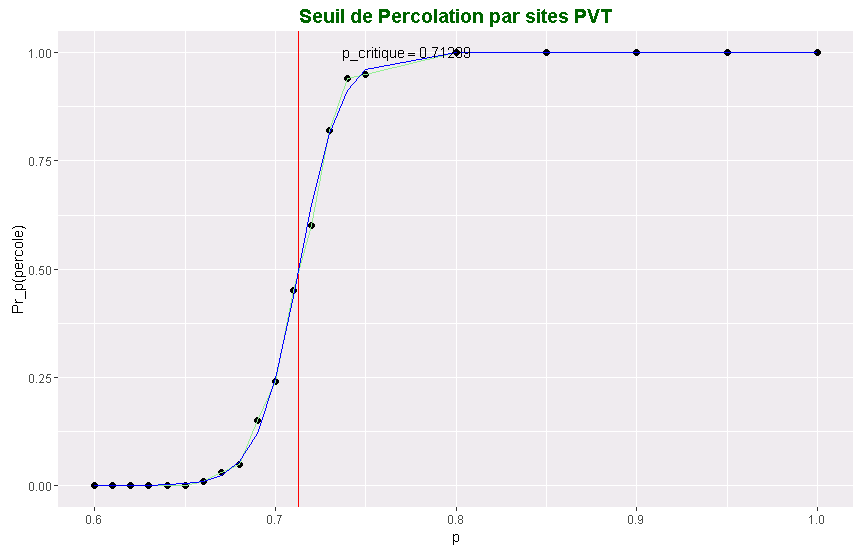
\includegraphics[width=0.48\linewidth]{Figures/Site-threshold-PVT}
\hspace{0.01\linewidth}
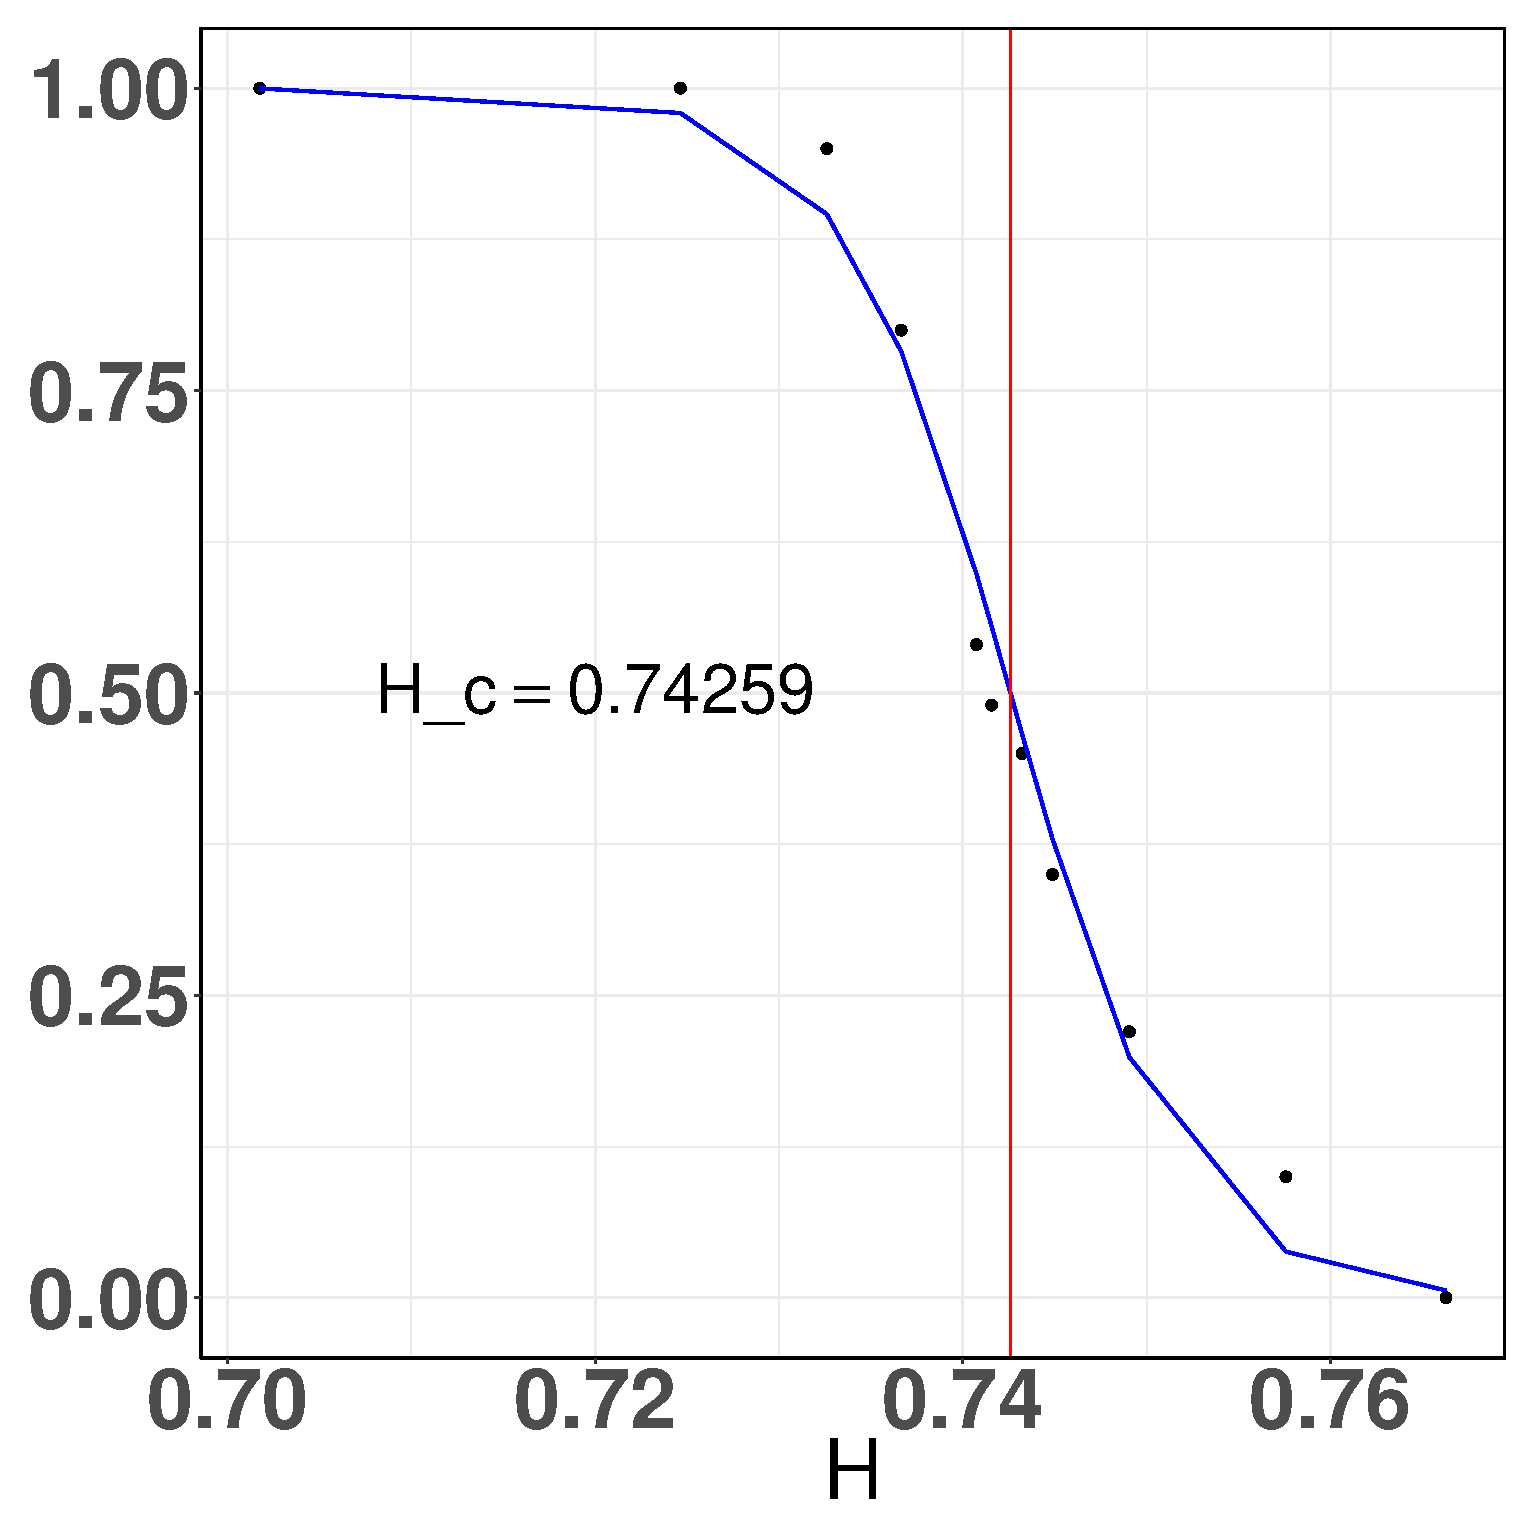
\includegraphics[width=0.48\linewidth]{Figures/sites-H_c-p=1}}
\centerline{\footnotesize\hspace{0.25\linewidth} (a)\hspace{0.5\linewidth} (b) \hspace{0.25\linewidth}\ }
\caption{Left: Estimation of $p_c$. Right: Estimation of $H_c$.
The black points are the discrete values of the probability of the window
crossing obtained by simulation (window size 30x30 $\text{km}^{2}$, street density $\gamma = 20 \; \text{km/km}^{2}$), the blue curve is the logistic model and the red vertical line is supposed to intercept the percolation threshold.}
\label{p-H-thresholds}
\end{figure}


\subsection{Relay-limited connectivity}
\label{ss.RelayLimited}
After having proven that there exists a minimal relay proportion under which no large-scale connectivity of the network is possible, regardless of all others network parameters, we may wonder whether connectivity of the D2D network can solely relying on relays. Indeed, with  the D2D communication range beging a physical constraint imposed by the type of D2D technology and link used \cite{asadi_survey_2014}, one can think  that if there are sufficiently many streets shorter than this range, a sufficiently high proportion of relays could  be  deployed allowing one  for long-range D2D communications even when the user density is low, i.e. $U \rightarrow 0$. 
This is indeed the case, as we shall see in what follows.
%The mathematical intuition behind this is the following: in a PVT, there is a positive probability of finding an arbitrarily long edge, but our simulation windows (as well as real environments) are bounded, or consisting in several morphologically homogeneous bounded zones \cite{courtat_promenade_2012}. Therefore, the maximum edge length in a bounded observation window is a bounded random variable with high probability. As a consequence, if the former maximum is not too large compared to the D2D communication radius (which corresponds to $H$ somehow small enough), a sufficiently large proportion of relays $p$ should therefore lead to percolation of $\mathcal{G}_{0,H,p}$, and therefore to percolation of $\mathcal{G}_{U,H,p}$ for any $U \leq 0$, as having users serving as D2D relays can only enlarge the number of connections, hence making percolation to occur more easily. \\

\indent For given $H$ (representing the ratio of the mean length of the typical steet to the D2D communication range), let us consider first  the best possible case where all crossroads are equipped with relays, i.e. $p=1$. If large-scale connectivity without users cannot be achieved when all crossroads are equipped with relays, then it also cannot be achieved for any $p \in (p_c,1)$. Setting $p=1$, define the following critical value for $H$: 
\begin{equation}
    \label{critical-H}
    H_{c}  \coloneqq \sup \lbrace H > 0, \; \mathcal{G}_{0,H,1} \; \text{percolates}\}\,.
\end{equation}
Possibility of percolation in the absence of users is equivalent 
verifying whether $H_c>0$. This theoretical question can be
answered affirmatively, and we approximate $H_c$ by simulations.


In this regard, we compute, for a grid of values of $H$, the proportion $g(H)$ of simulations where the graph $\mathcal{G}_{0,H,1}$ percolates. Here, a generalized logistic model \textbf{Name of the inverse S shaped curve?} yields a good fitting of the estimated curve, see Figure~\ref{p-H-thresholds}(b). Finally, we recover $H_{c}$ by the abscissa of the inflection point of the logistic curve and find the following estimate: $H_c \approx 0.743$. \\

\indent In the remaining part of this section we investigate the 
the relay-limited connectivity regime 
when $H < H_c$, that is when there is a possibility of percolation in the absence of users. The question is whether we need for this the complete deployment of  
relays ($p=1$), as assumed in~\eqref{critical-H}.
The intuition is that statistically shorter streets (corresponding $H<H_c$) might require only some proportion of crossroads equipped with relays. In mathematical terms we define the following critical proportion of relays ensuring percolation of the connectivity graph $\mathcal{G}_{0,H,p}$ in the absence of users in the relay-limited connectivity regime  $H<H_c$
\begin{equation}
    \label{p_c(H)}
    p_c(H) \coloneqq \inf \lbrace p>(0,1) \; \mathcal{G}_{0,H,p} \; \text{percolates}. \rbrace
\end{equation}
We already know from Section~\ref{relay-influence} that 
$p_c(H)\ge p_c$ and it can be proved mathematically that $p_c(H)<1$ for all $H<H_c$. Our goal is again to approximated this function by simulation.

The methodology is quite the same as in the previous numerical simulations: this time, for a given $H<H_c$ and a grid of values of $p \in (p_c,1)$, we compute the proportion $k(p)$ of simulations where the graph $\mathcal{G}_{0,H,p}$ percolates. Theory tells us that $k$ is increasing in $p$ (more relays indeed implies more connections, hence making percolation easier to occur) and logistic model again yields a good fitting of the estimated curve and leads to $p_c(H)$ as the inflection point of the logistic curve. The estimated values are presented in Table~\ref{tab-p_c(H)}. As can easily be guessed and as is confirmed by our results $p_c(H)$ is increasing with $H$.
We were able to consider only  $H>0.46$. Below this value 
the system started having an erratic behaviour not giving any  
reasonable estimation of $p_{c}(H)$. This can be explained by the  fact
that when $H$ approaches~0, $p$ approaches $p_{c}$ and the simulation of the model close to critically is much more tricky.
%and the relay proportion is not sufficient anymore to allow for site percolation on a large proportion of the simulated graphs (as shown in Fig.\ref{site-threshold}, the estimated percolation probability quickly decreases in the window $\left[0.72,0.74\right]$). By Theorem \ref{minimality_theorem}, if the graph $\tilde{\mathcal{G}}_{p}$ associated with the Bernoulli site percolation on $S$ does not percolate, then neither does $\mathcal{G}_{0,H,p}$. An additional explanation relies on the assumption (strongly believed to be true by analogy with the well-known Poisson Boolean model \cite{blaszczyszyn_stochastic_2018}) that the infinite connected component of $\mathcal{G}_{0,H,p}$ is almost surely unique. Therefore, for percolation of $\mathcal{G}_{0,H,p}$ to occur, the exact precise street segments belonging to the almost surely unique connected path crossing the simulation window have to let communications through, i.e. have relays present at their both endpoints. When $p$ approaches $p_{c}$, the former becomes very unlikely.



\begin{remark}
In practice, operators have leverage on $p$ (by equipping more or less crossroads with relays). The results provided in Table~\ref{tab-p_c(H)}
allow them to find appropriated proportion of relays
in function of  $H$, which depends both on the D2D technology and the inner geometry of the network. In this table we also relate $H$ to  D2D communication range $r=\frac{4}{3}\frac{1}{H\gamma}$  (see Eq.\eqref{dimensionless-parameters}) in case of an urban environment taking $\gamma = 20 \, \text{km/km}^{2}$. 
It is worth noticing that the  relay-limited connectivity regime 
($H < H_c$)  in this environment implies  $r$ smaller  than 150 meters, a technological threshold which does not seem physically unreachable. \cite{lin_comprehensive_2013}. 
\end{remark}
\begin{table}[t!]
\caption{Critical parameter $p_{c}(H)$ and corresponding $r$ in an urban environment as a function of $H$}
\begin{center}
\begin{tabular}{|c|c|c|}
\hline
$H$ & $p_c(H)$ & $r$ (meters), urban environment \\
\hline
0.467 & 0.75 & 142.96  \\
0.487 & 0.76 & 136.96 \\
0.503 & 0.77 & 132.60 \\
0.521 & 0.78 & 127.95  \\
0.534 & 0.79 & 124.90 \\
0.548 & 0.80 & 121.72  \\
0.609 & 0.85 & 109.52 \\
0.655 & 0.90 & 101.75 \\
0.702 & 0.95  & 95.03 \\
$H_c \approx 0.743$ & 1 & 89.78  \\
\hline
\end{tabular}
\label{tab-p_c(H)}
\end{center}
\end{table}
\begin{figure}[t!]
\centering
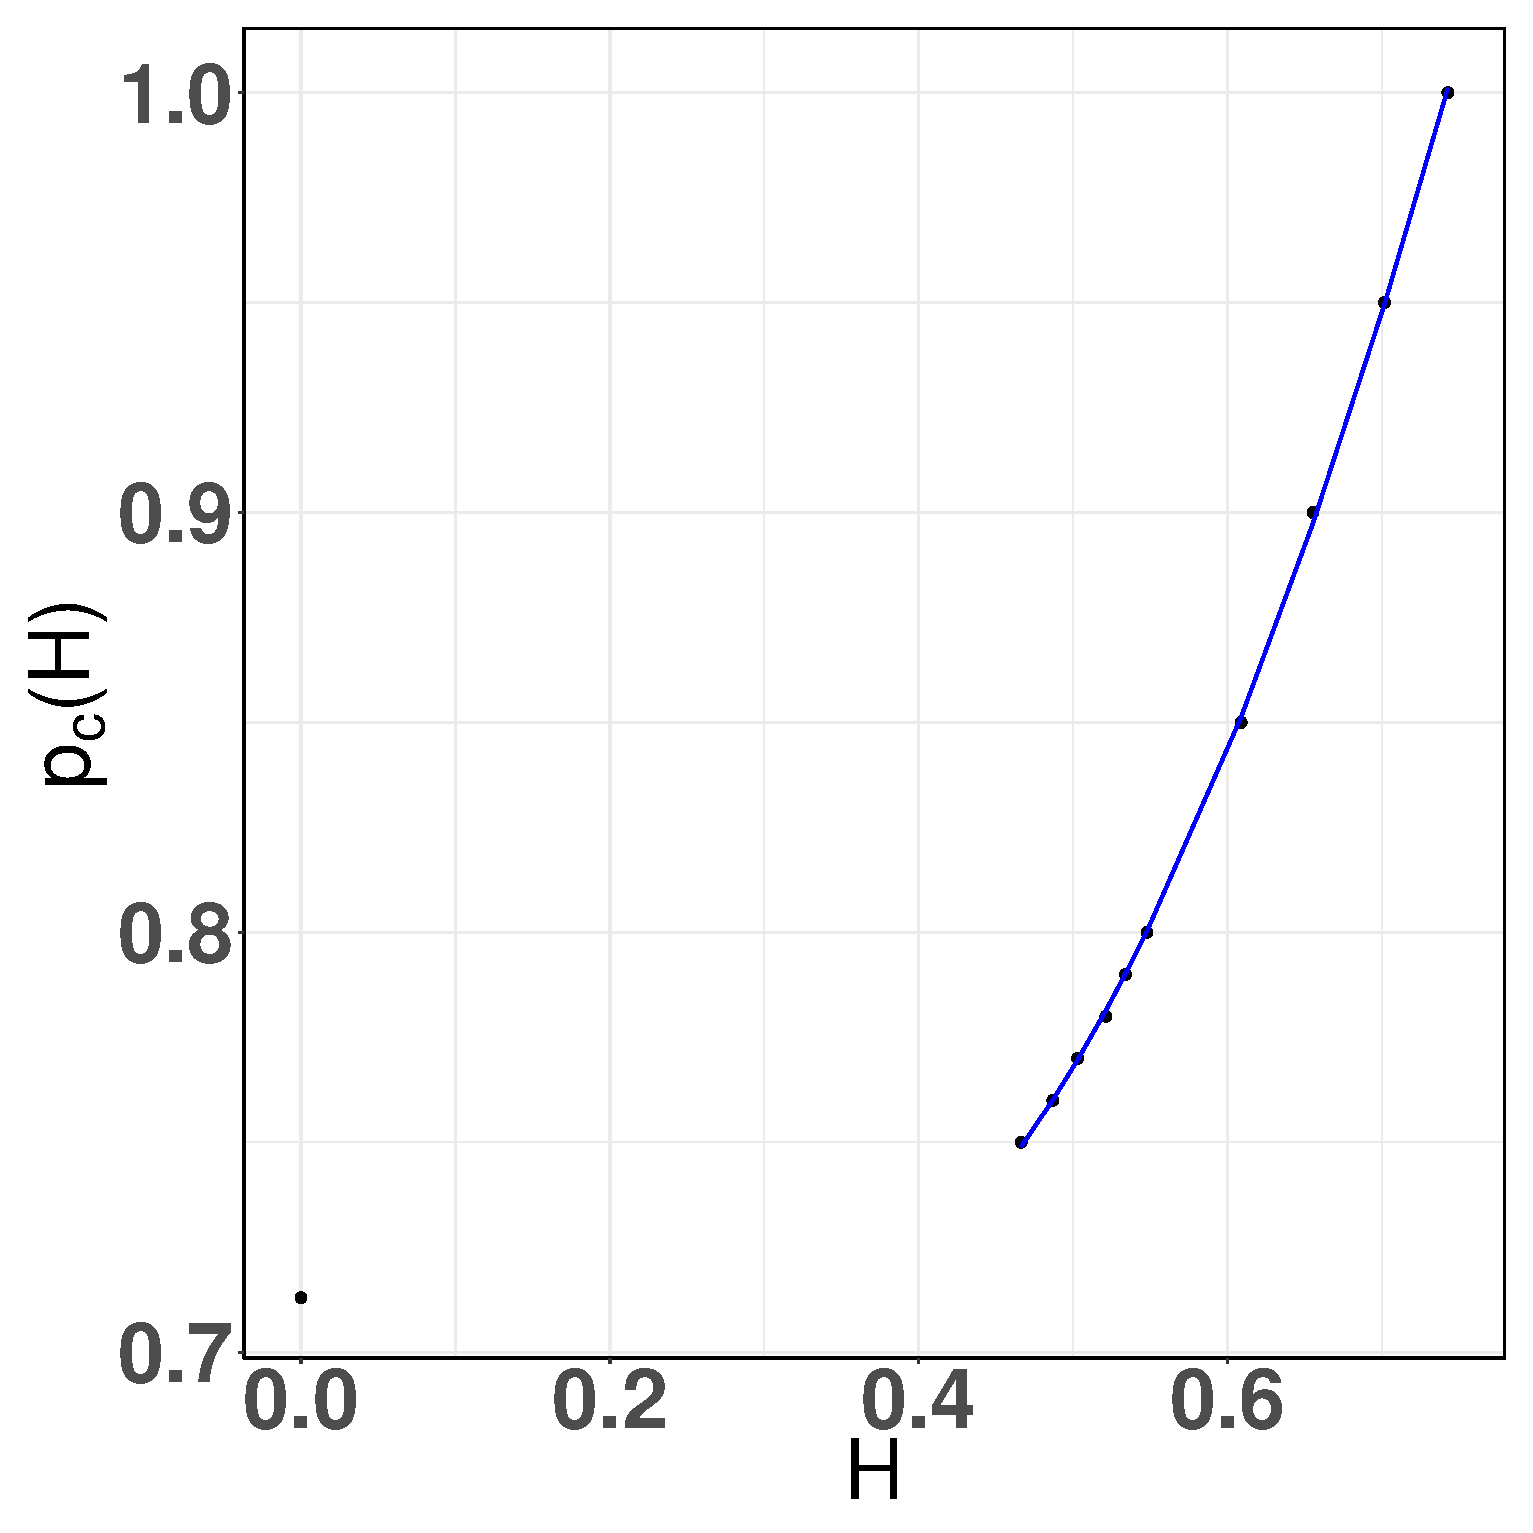
\includegraphics[width=0.60\linewidth]{Figures/pcH}
\caption{Critical relay proportion $p_c(H)$ in the absence of users ($U=0$) as a function of $H$. The black points are the discrete points from Table~\ref{tab-p_c(H)}, the blue curve is the estimated quadratic fit.
The isolated point $p_c(0)=p_c$ corresponds to the (absolute) minimal relay proportion~\eqref{e.pc}. }
\label{quadratic-fit-p_c(H)}
\end{figure}


\indent  In order to get a continuous approximation for $p_c(H)$ for $0.46<H<H_c$ we interpolate the discrete values given in Table~\ref{tab-p_c(H)}. 
We found out that the following quadratic model %given by \eqref{quadratic-model} 
\begin{equation}
\label{quadratic-model}
p_c(H) \approx aH^{2} + bH + c
\end{equation}
with the  value of the coefficients $a$, $b$ and $c$ estimated by linear regression
$a \approx 1.45$, $b \approx -0.84$, $c \approx 0.83$
yields a good fit able to explain 99\% of the variance. Fig.\ref{quadratic-fit-p_c(H)} illustrates the discrete simulated curve and the estimated quadratic fit for $p_c(H)$, confirming that a quadratic model is a very good approximation.


\subsection{Relay-and-user-limited connectivity}
\label{ss.Relay-and-Users}
The main question arising from the previous section is about what happens when the D2D range and the street system do not allow to reach the critical parameter $H_c$ and thus to solely rely on relays for ensuring large-scale connectivity of the network. In other words, for $H>H_c$ is there a critical user density above which long-range communications are possible? If so, which minimal relay proportion is appropriate for ensuring large-scale connectivity with the help of users serving as D2D relays? \\
\indent As in Section~\ref{ss.RelayLimited}, for some $H>H_c$, let us consider first the case where $p=1$. If large-scale connectivity relying on both users and relays cannot be achieved when all crossroads are equipped with relays, then it also cannot be achieved for any $p \in (p_c,1)$. Setting $p=1$ and for given $H>H_c$, define the following critical value for $U$:
\begin{equation}
\label{critical-U}
U_c(H) \coloneqq \inf \lbrace U \geq 0, \; \mathcal{G}_{U,H,1} \; \text{percolates} \rbrace  
\end{equation}
The numerical results from Section \ref{ss.RelayLimited} ensure that for $H<H_c$, we have $U_c(H)=0$. We are therefore interested in the case where and $H>H_c$. In particular, do we have $0 < U_{c}(H) < \infty$ ? 

\subsubsection{Non-triviality of the critical parameter $U_c(H)$}
On a theoretical perspective, we were able to prove that under sufficiently general conditions, the critical parameter $U_c(H)$ representing the minimal average number of users per typical street allowing for long-range communications is indeed positive and finite. Our two main results are the following ones:
\\
\begin{theorem}[Positivity of $U_c(H)$]
%Shall I mention again that S is a PVT, hence stabilising and essentially asymptotically connected?
\label{positivity-critical-U}
Assume $H>H_c$. Then there exists an absolute constant $H^{*} \geq H_c$, possibly different from $H_c$, such that whenever $H > H^{*}$, $U_c(H)>0$. In other words, long-range communications cannot be achieved in the absence of users if the streets of the network are large compared to the D2D range. \\
\end{theorem}
\begin{theorem}[Finiteness of $U_c(H)$]
%same here
\label{finiteness-critical-U}
Assume $H > H_c$. Then we have $U_c(H) < \infty $. In other words, long-range communications can be achieved under a sufficiently high (but finite!) user density, even if the streets of the network are large compared to the D2D range.
\end{theorem}
\indent As the goal of this paper is more about giving numerical estimates, rigorous proofs of Theorems \ref{positivity-critical-U} and \ref{finiteness-critical-U} will be provided in a companion paper to be published in a mathematical journal. We therefore only give rough sketches of the former proofs and omit tedious technical details. Both proofs crucially rely on the fact that the chosen street system $S$ is a PVT and is therefore stabilizing and asymptotically essentially connected, as explained and proven in \cite{hirsch_continuum_2017}. 
%talk about renormalisation arguments here? Moreover, they appeal to so-called renormalisation techniques \cite{blabla}, which consist in introducing on the same underlying geometry that the one we used a discrete percolation problem, easier to solve than a continuous one... 
\\

\begin{IEEEproof}[Sketch of proof of Theorem \ref{positivity-critical-U}]
The idea behind stabilization is that the configuration of the network environment in a given observation window only depends from a bounded region including the observation window with high probability. In other words, if two observed regions of the network are sufficiently distant, they are independent. This allows to introduce a discretized site percolation process featuring short-range spatial dependencies only. Well-chosen definitions of open and closed sites in the former process allow to ensure that if the discretized process does not percolate, then neither does $\mathcal{G}_{U,H,1}$. Finally tedious technical details based on the use of the domination by product measures theorem \cite{liggett1997domination} allow to conclude that the discretized process does not percolate if $U$ is sufficiently small and $H > H^{*}$ for some absolute constant $H^{*}\geq H_c$ ($H^{*}$ only depends on the edge length distribution of the edges in a PVT). Hence, our original process does not percolate if $U$ is sufficiently small and $H > r^{*}$. Therefore, $U_{c}(H) > 0$ whenever $H > H^{*}$, which concludes the proof.
\end{IEEEproof}

\vspace{1\baselineskip}

\begin{IEEEproof}[Sketch of proof of Theorem \ref{finiteness-critical-U}]
The techniques used in this proof are similar to the ones used in the proof of Theorem \ref{positivity-critical-U}. In this case, we introduce a discrete percolation process chosen so that if the former process percolates, then so does $\mathcal{G}_{U,H,1}$. Crucially relying on the asymptotic essential connectedness \cite{hirsch_continuum_2017} of the PVT street system $S$ and using again the domination by product measures theorem \cite{liggett1997domination} allows to conclude that the discretized percolation process percolates if $U$ and $H$ are sufficiently large. Hence the result.
\end{IEEEproof}

\vspace{1\baselineskip}

\subsubsection{Numerical estimations of $U_c(H)$}
On a more applied note and in the light of the results given by Theorems \ref{positivity-critical-U} and \ref{finiteness-critical-U}, it also is of great interest, especially for operators willing to study the technical feasibility of a D2D-enabled network, to get numerical estimates of the critical parameter $U_c(H)$, corresponding to the minimal average number of user per typical street needed to ensure large-scale connectivity of the network. This is the issue we tackle in this subsection. \\
\indent The simulation method used to estimate $U_{c}(H)$ for given $H$ is merely the same as in Sections \ref{relay-influence} and \ref{ss.RelayLimited}: for a given $H$ and a grid of values for $U$, we simulate a large number of connectivity graphs $\mathcal{G}_{U,H,1}$ and compute the proportion $l(U)$ of simulations where $\mathcal{G}_{U,H,1}$ percolates. Again, a logistic model gives a good fitting of the estimated curve, and we determine $U_{c}$ by noting the abscissa of the inflection point of the logistic curve. Fig.\ref{critical-user-estimation}(a) illustrates an example for $H \approx 0.89$ (corresponding to a D2D range $r = 75 \text{m}$). We also provide our simulated curve for $U_c(H)$ as function of $H$ in Fig.~\ref{critical-user-estimation}(b): for time-constraint reasons, we were only able to obtain a few values of $U_c(H)$ given by the black points. Note that $U_c(H) = 0$ whenever $H < H_c \approx 0.743$ and that $U_c(H)$ seems to behave almost linearly as a function of $H$.
\begin{figure}[t!]
\centerline{
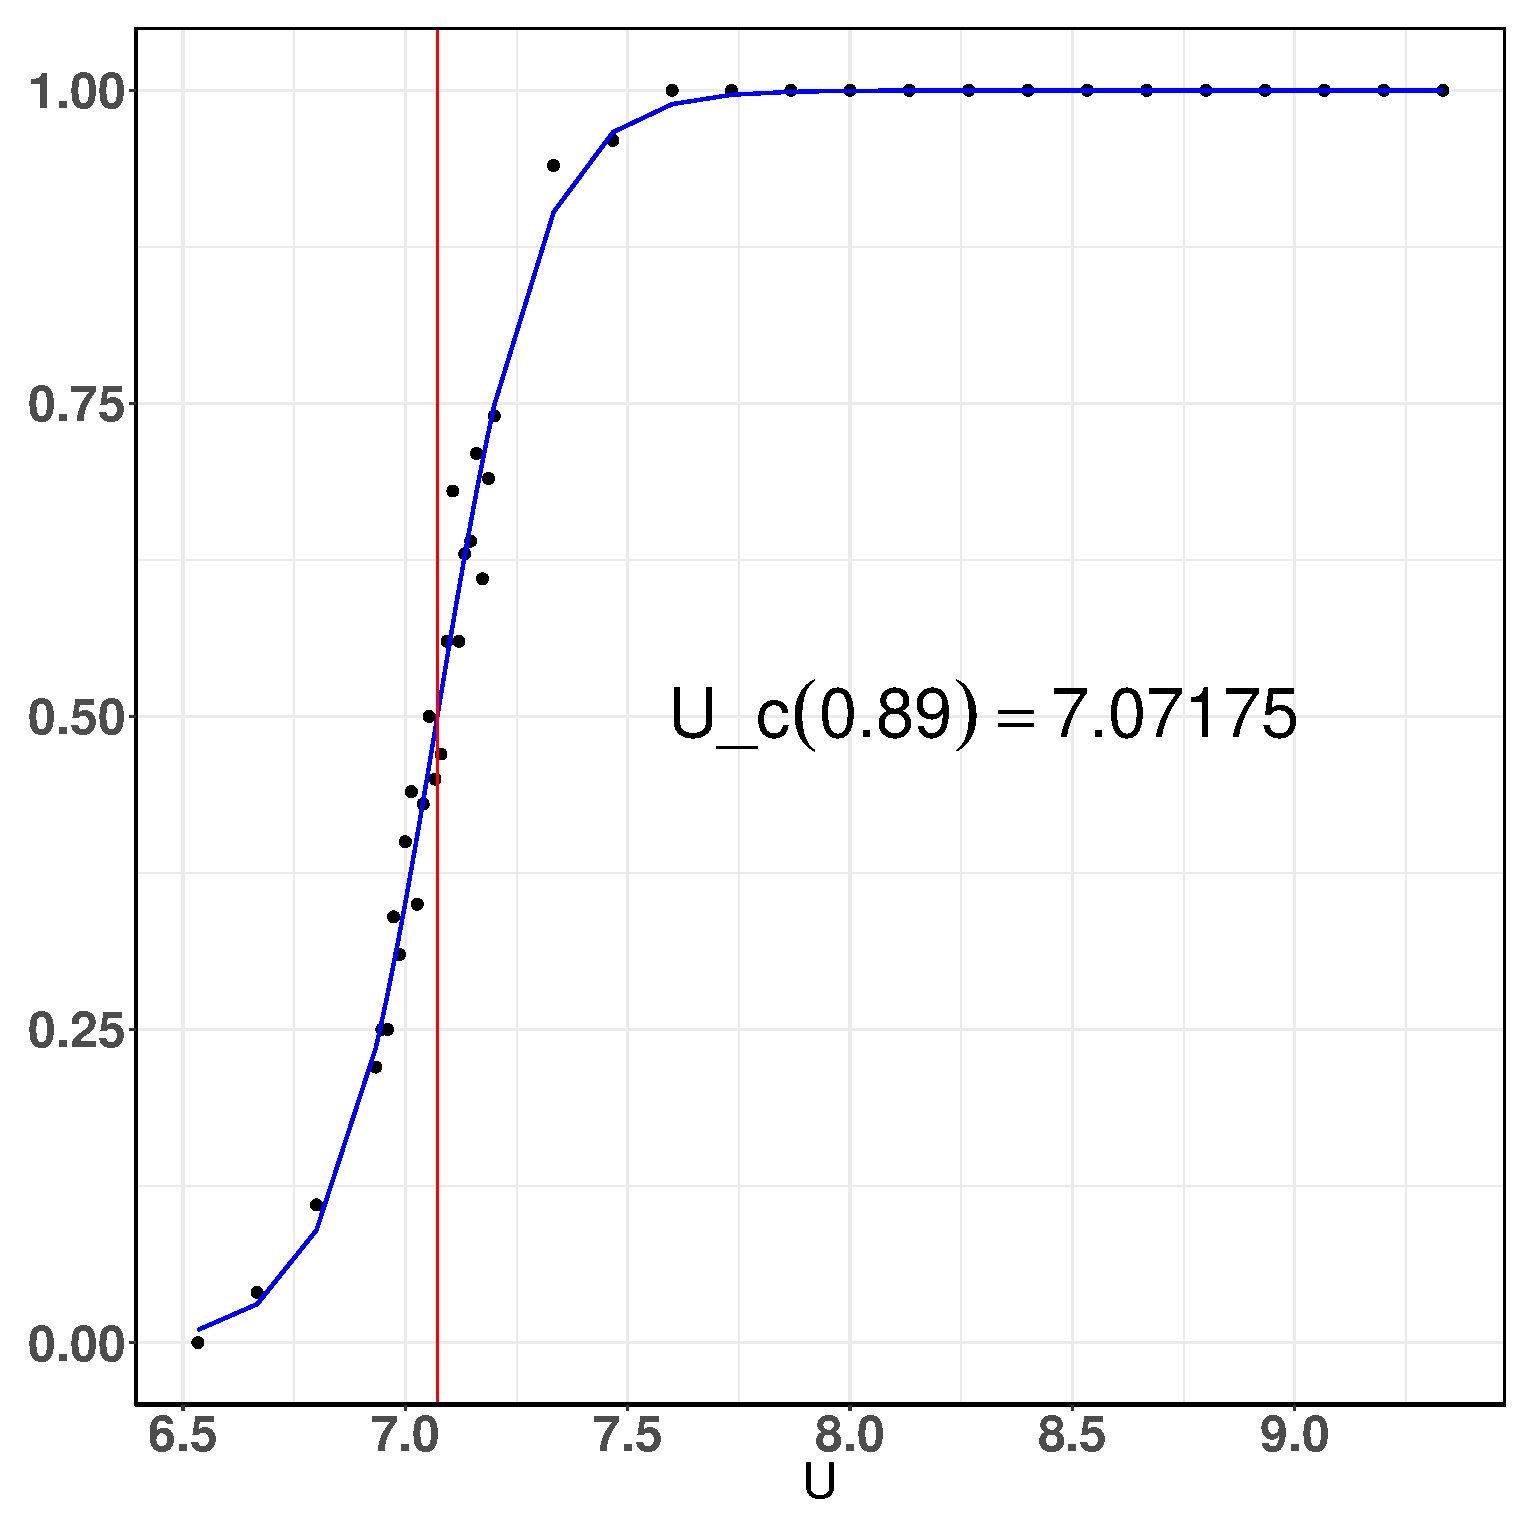
\includegraphics[width=0.48\linewidth]{Figures/Uc-example}
\hspace{0.01\linewidth}
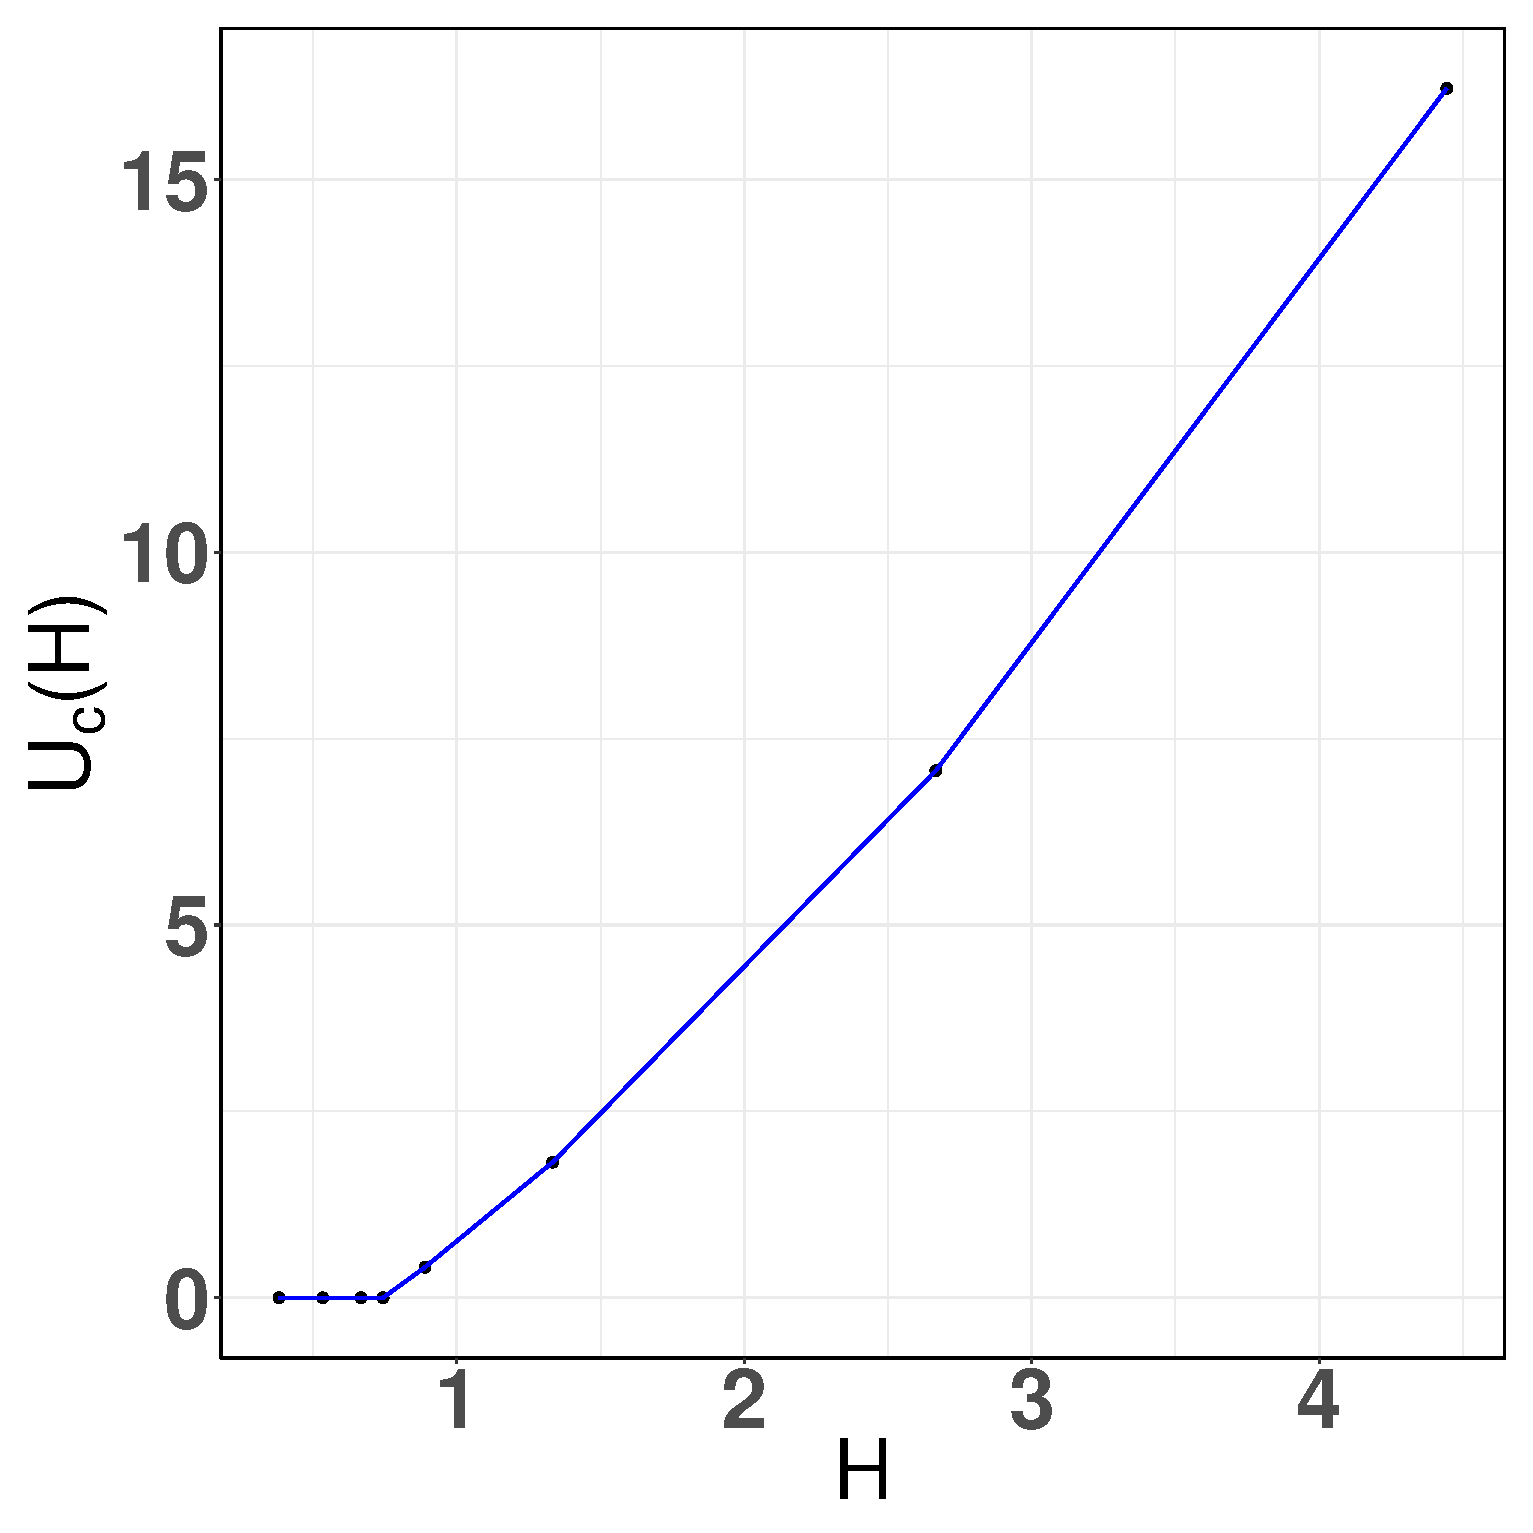
\includegraphics[width=0.48\linewidth]{Figures/Uc-general-curve}}
\centerline{\footnotesize\hspace{0.25\linewidth} (a)\hspace{0.5\linewidth} (b) \hspace{0.25\linewidth}\ }
\caption{Left: Estimation of $U_{c}(H)$ for $H\approx 0.89$. The simulation window is of size 10x10 $\text{km}^{2}$ for time-constraint purposes. The black points are the discrete values of $l(U)$ obtained by simulations, the blue curve is the logistic model and the red vertical line determines the intercept $U_{c}(H)$. Right: $U_c(H)$ as a function of $H$.}
\label{critical-user-estimation}
\end{figure}

\vspace{1\baselineskip}
From the results in Sections~\ref{ss.RelayLimited} and ~\ref{ss.Relay-and-Users}, we have seen that users and relays have to compensate each other to allow for arbitrarily long-range communications on the network whenever $H>H_c$. In fact, even when large-scale connectivity can solely be ensured by relays, i.e. $H<H_c$, an operator might rather want to invest less in relays and incentivize users to serve as D2D relays. The compromise between relay proportion and user density can be captured by either of the following functions:
\begin{itemize}
    \item $(U,H) \mapsto p_c(U,H) \coloneqq \inf \lbrace p>p_c, \; \mathcal{G}_{U,H,p} \; \text{percolates} \rbrace$
    \item $(p,H) \mapsto U_c(p,H) \coloneqq \inf \lbrace U \geq 0, \; \mathcal{G}_{U,H,p} \; \text{percolates} \rbrace$
\end{itemize}
In this regard, we chose the second option and shall present in the next section some values of $U_c(p,H)$ for both regimes $H<H_c$ and $H>H_c$.
\begin{remark}
\label{remark-inverse-Uc(p,H)}
Both approaches are actually equivalent and choosing either one is just a matter of convenience and practicality for numerical simulations. Indeed, it can be mathematically be proven that $U_c(p,H)$ is an increasing function of $p$ for fixed $H$ and can hence be inverted: this leads back to the critical relay proportion $p_c(U,H)$.
\end{remark}
\subsection{Critical user density  in relay augmented D2D network}
For given $p>p_c$ and $H >0$, the function $(p,H) \mapsto U_c(p,H)$ can be seen by an operator as an indicator on the average number of users needed for a given investment relays so as to successfully deploy a D2D network. Note that the function $U_c(H)$ defined in \eqref{critical-U} is such that: $\forall H>H_c, U_c(H) = U_c(p=1,H)$. The interest of computing $U_c(p,H)$ also when $H<H_c$ relies on the fact that an operator might rather want to rely on its already existing subscribers than on new relays.\\
\indent The simulation method used to estimate the critical average number of users $U_{c}(p,H)$ is merely the same as in Section~\ref{ss.Relay-and-Users}: for given $p>p_c$ and $H$ and a grid of values for $U$, we simulate a large number of connectivity graphs $\mathcal{G}_{U,H,p}$ and compute the proportion $m(U)$ of simulations where $\mathcal{G}_{U,H,p}$ percolates. Again, a logistic model gives a good fitting of the estimated curve, and we determine $U_{c}(p,H)$ by noting the abscissa of the inflection point of the logistic curve. Fig.~\ref{critical-user-estimation-twovar}(a) illustrates an example. Results for estimations of $U_c(p,H)$ are given in Table \ref{tab-critical-U}, where we also include a comparison with results from \cite{cali2018percolation}, where the authors simulated a model similar to ours without any shadowing effects (NoSha), i.e. there are only users on streets distributed according to a Cox process and any two users (being in LOS or in NLOS) with reciprocal Euclidean distance less than $r$ are connected. It is clear from Table \ref{tab-critical-U} that the previous estimates from \cite{cali2018percolation} are much smaller than ours: taking the canyon shadowing assumption into account in our model indeed provides more realistic information for operators.

%\begin{figure}[t!]
%\centering
%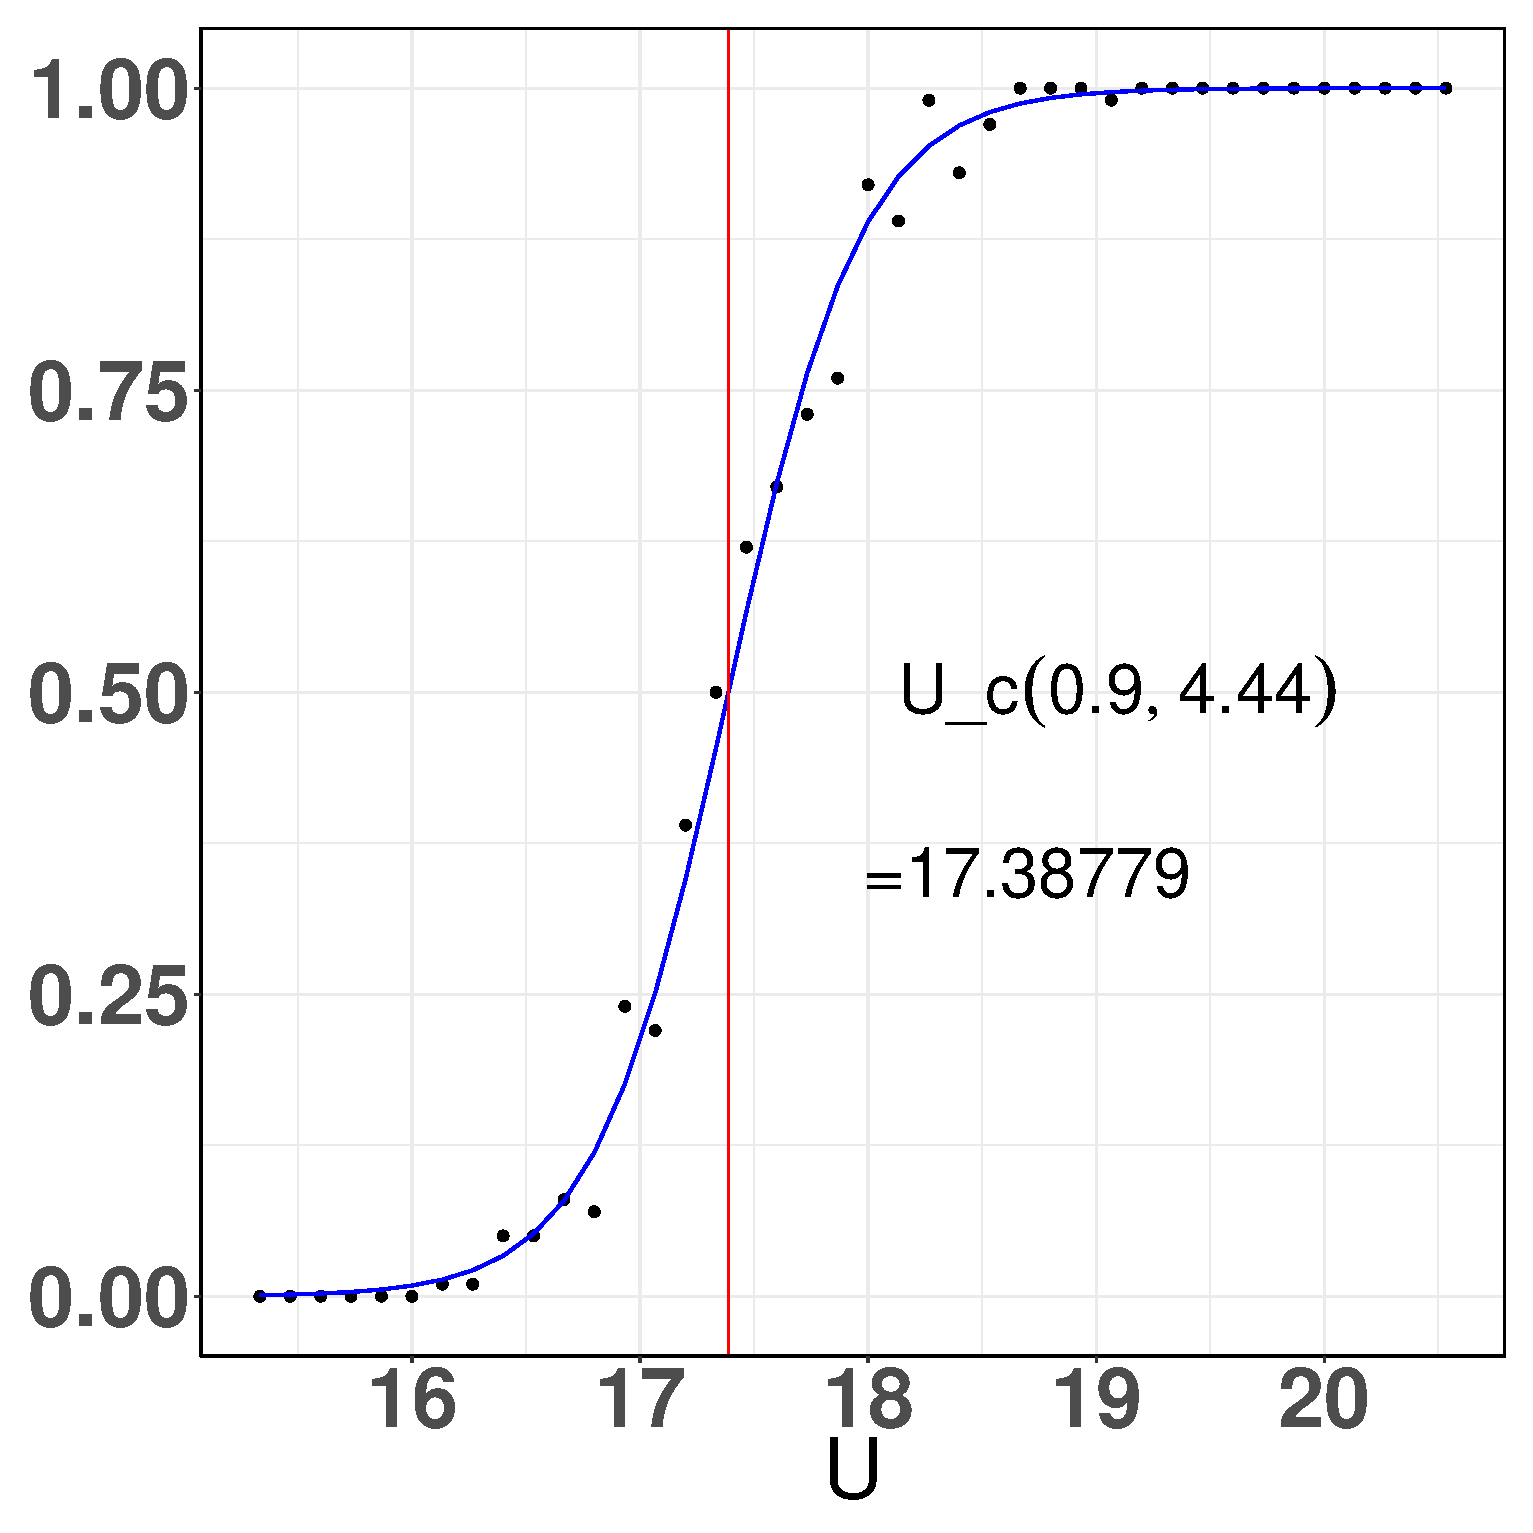
\includegraphics[width=0.48\linewidth]{Figures/Uc-twovar-example}
%\caption{Estimation of $U_{c}(p=0.9,H \approx 4.44)$, corresponding to $r=15 \, \text{m}$ in an urban environment ($\gamma = 20 \, \text{km/km}^{2}$). The simulation window is of size 10x10 $\text{km}^{2}$ for time-constraint reasons. The black points are the discrete values of $m(U)$ obtained by simulations,  the blue curve is the logistic model and the red vertical line determines the intercept $U_{c}(p,H)$.}
%\label{critical-user-estimation-twovar}
%\end{figure}

\begin{figure}[t!]
\centerline{
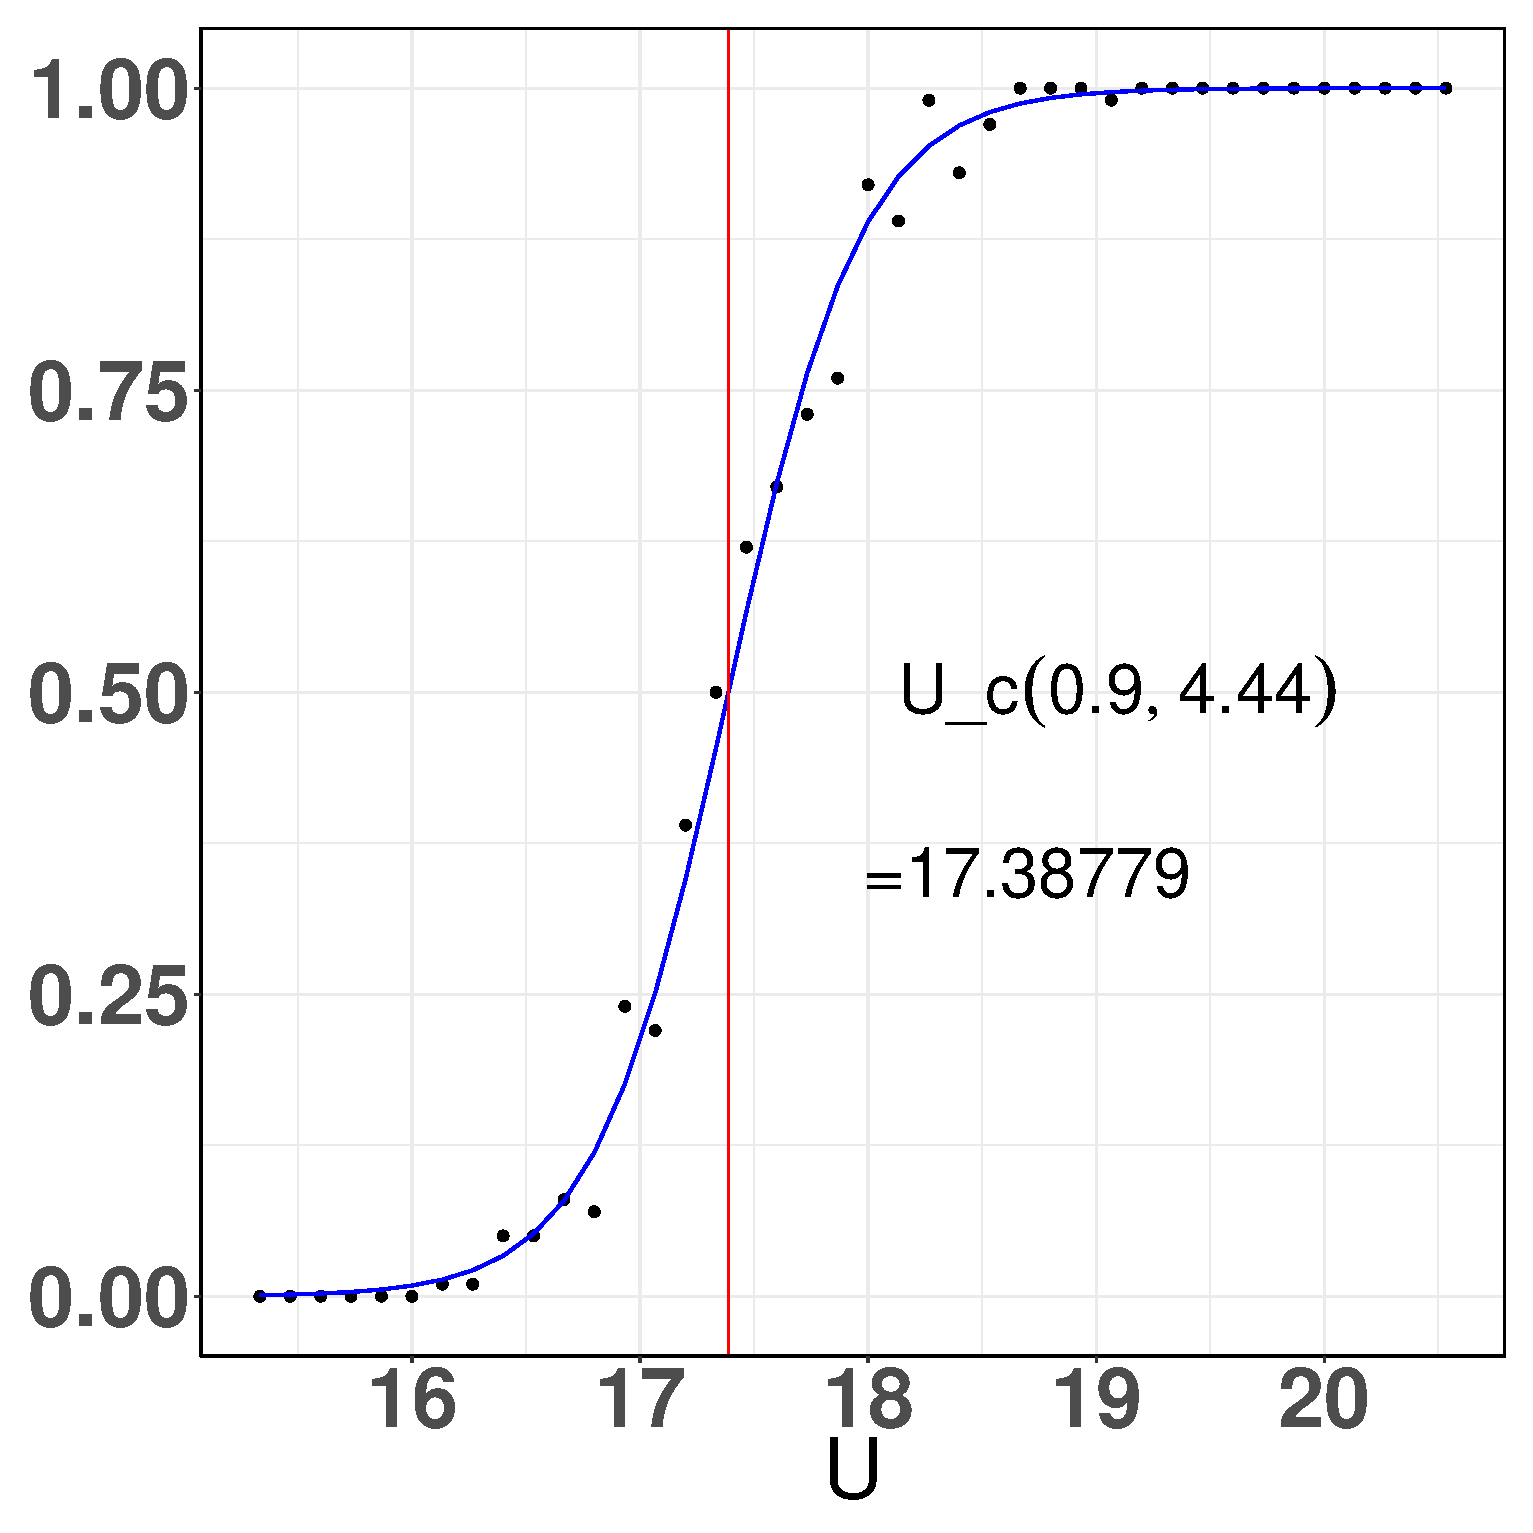
\includegraphics[width=0.48\linewidth]{Figures/Uc-twovar-example}
\hspace{0.01\linewidth}
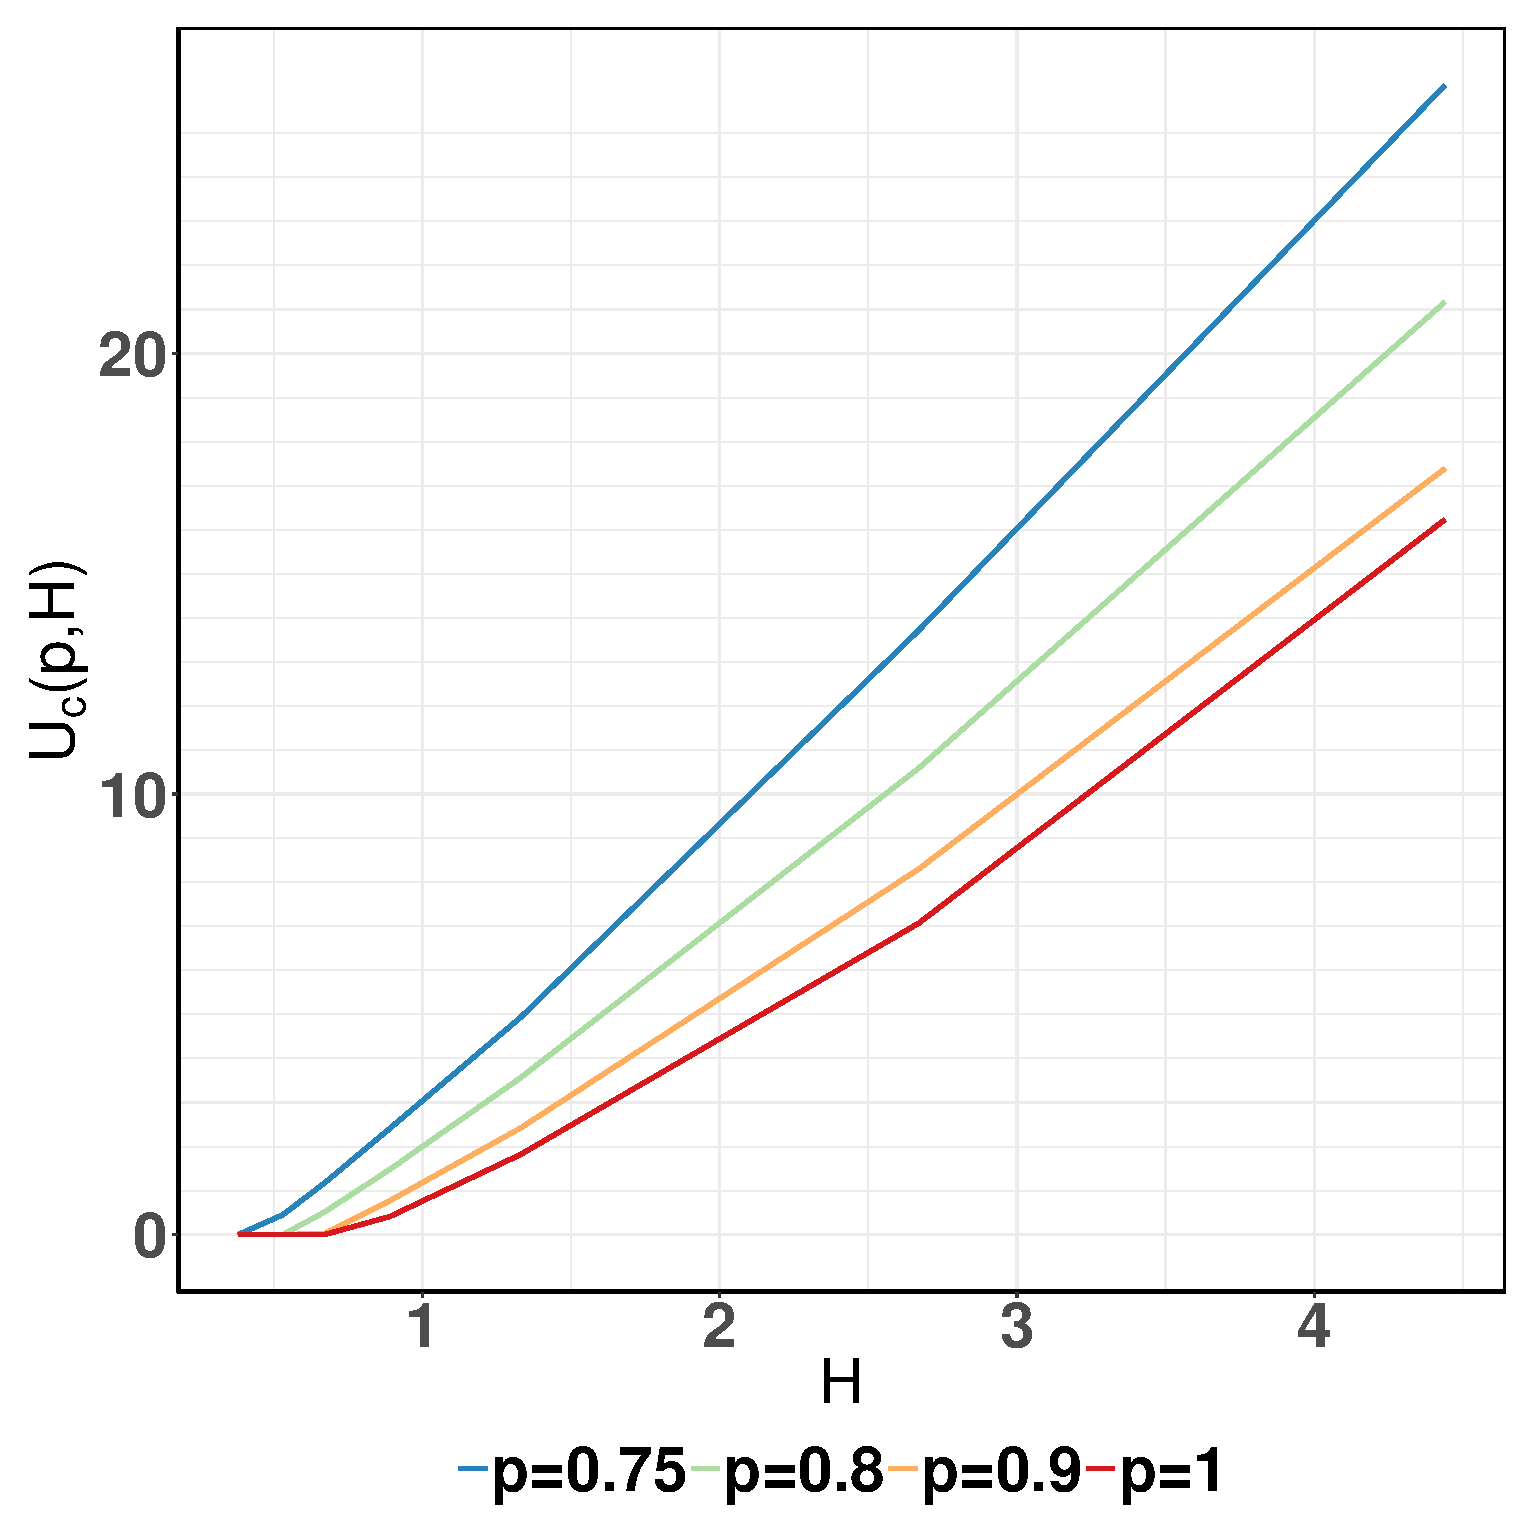
\includegraphics[width=0.48\linewidth]{Figures/critical-U-several-p}}
\centerline{\footnotesize\hspace{0.25\linewidth} (a)\hspace{0.5\linewidth} (b) \hspace{0.25\linewidth}\ }
\caption{Left: Estimation of $U_{c}(p=0.9,H \approx 4.44)$, corresponding to $r=~15 \, \text{m}$ in an urban environment ($\gamma = 20 \, \text{km/km}^{2}$). The simulation window is of size 10x10 $\text{km}^{2}$ for time-constraint reasons. The black points are the discrete values of $m(U)$ obtained by simulations,  the blue curve is the logistic model and the red vertical line determines the intercept $U_{c}(p,H)$. Right: Critical user density $U_c(p,H)$ as a function of $H$ for several values of $p$.}
\label{critical-user-estimation-twovar}
\end{figure}

\begin{table}[t!]
\caption{Critical user density $U_{c}(p,H)$ as a function of $p$ and $H$. NA stands for Non Applicable data in \cite{cali2018percolation}.} 
\begin{center}
\begin{tabular}{|c|c|c|c|c|c|}
\hline
\multicolumn{6}{|c|}{$U_c(p,H)$}\\
\hline
$H$ & $p=1$ & $p=0.9$ & $p=0.8$ & $p=0.75$ & NoSha \cite{cali2018percolation} \\
\hline
4.44 & 16.23 & 17.39 & 21.17  & 26.09 & 15.87 \\
2.67 & 7.07  & 8.30 & 10.59 & 13.72 &  7.44 \\
1.33 & 1.82 & 2.42 & 3.56 &  4.93 &  NA \\
0.89 & 0.41  & 0.77 & 1.48 & 2.41 &  1  \\
0.67 & 0  & 0.03 & 0.51 &  1.17 &  NA \\
0.53 & 0  & 0 & 0 & 0.45 & 0.32 \\
0.38 & 0 & 0 & 0 & 0 & 0.16 \\
\hline
\end{tabular}
\label{tab-critical-U}
\end{center}
\end{table}

%\begin{figure}[t!]
%\centering
%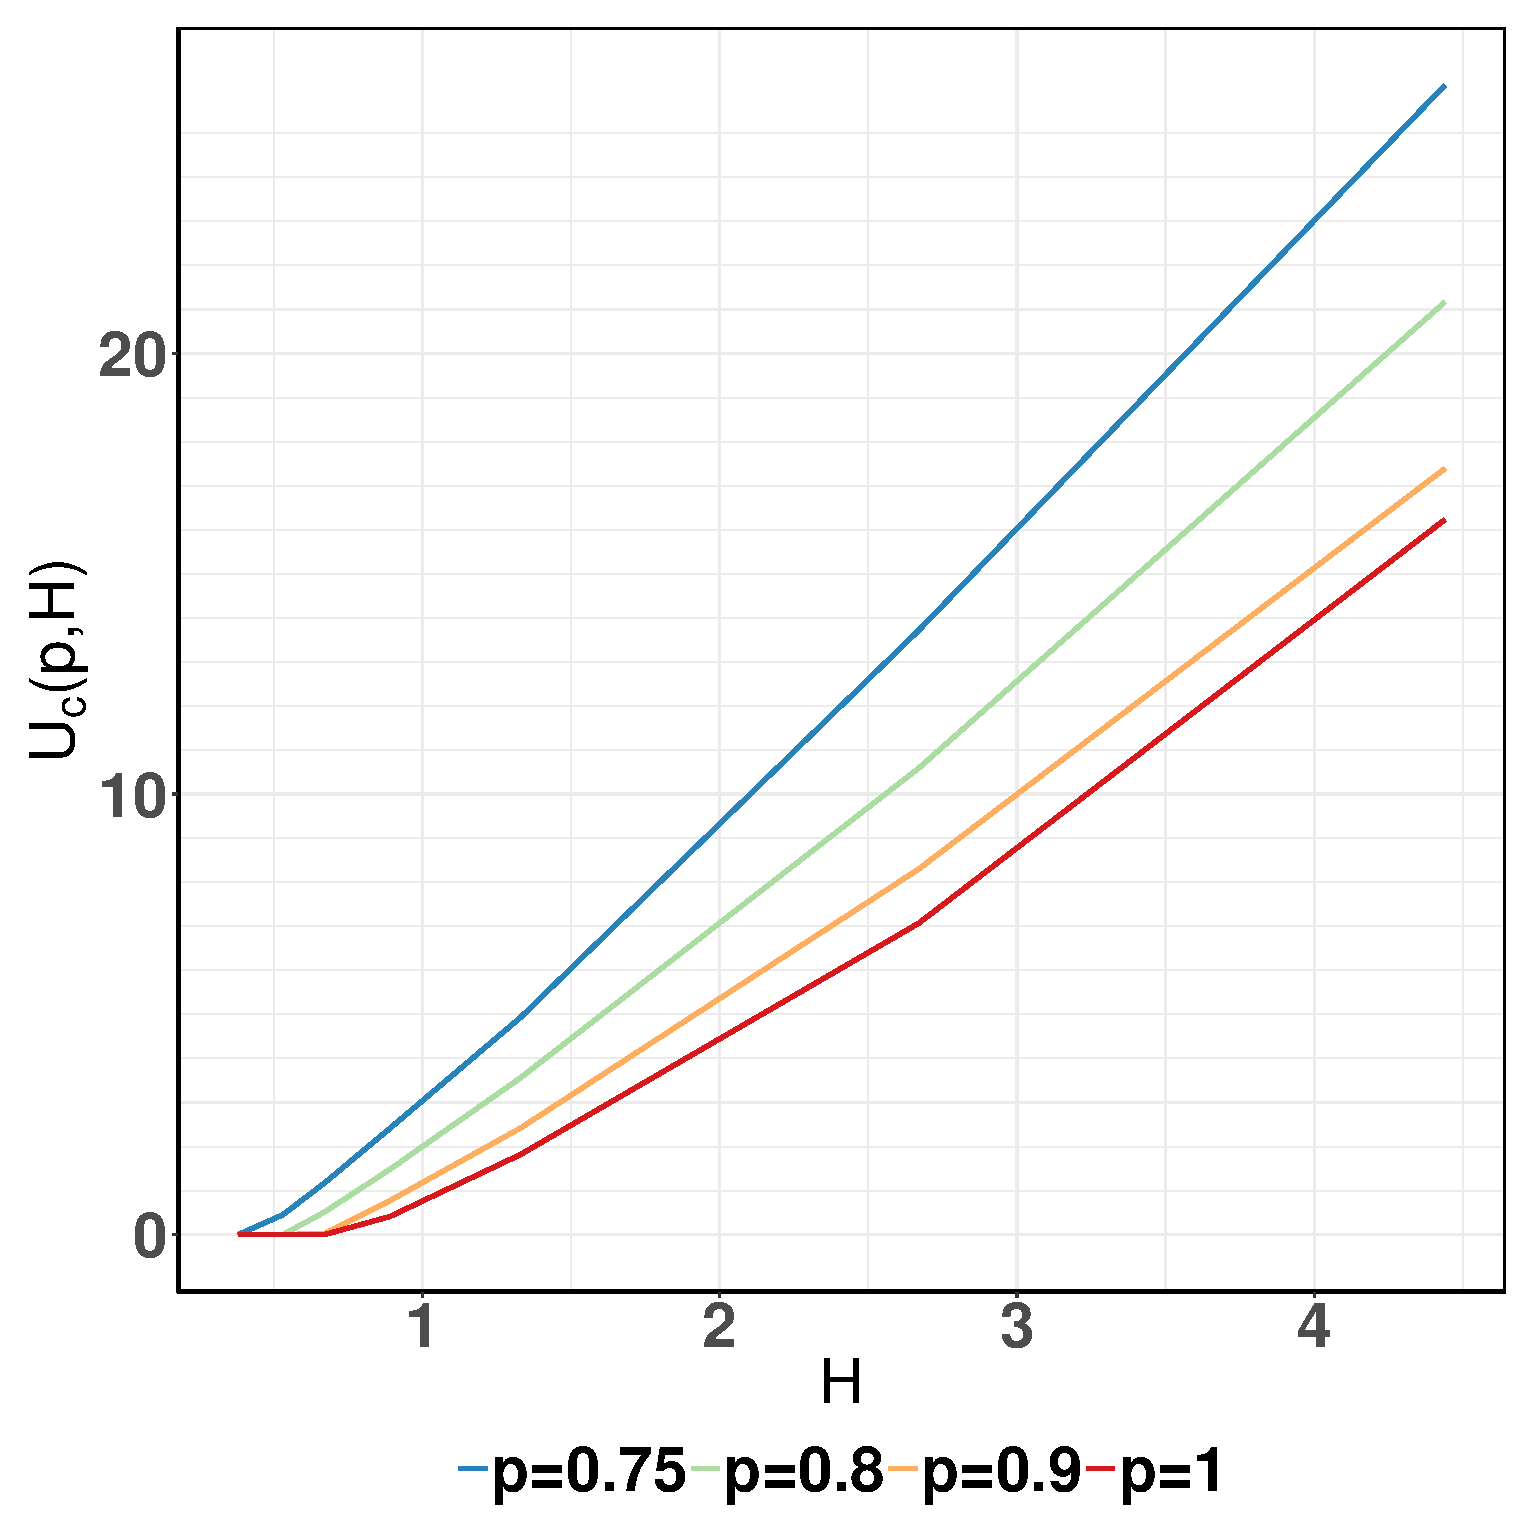
\includegraphics[width=0.48\linewidth]{Figures/critical-U-several-p}
%\caption{Critical user density $U_c(p,H)$ as a function of $H$ for several values of $p$.}
%\label{critical-density-comparison}
%\end{figure}
\indent Fig.~\ref{critical-user-estimation-twovar}(b) shows the variation of the critical user density $U_c(p,H)$ as a function of $H$ for several values of $p$. It is clear from Fig.~\ref{critical-user-estimation-twovar}(b) and Table \ref{tab-critical-U} that $H \mapsto U_c(p,H)$ is increasing for fixed $p$ and that $p \mapsto U_c(p,H)$ is also increasing for fixed $H$, which confirms the comment we made in Remark \ref{remark-inverse-Uc(p,H)}: for given $H$, we can inverse $U_c(p,H)$ to get back $p_c(U,H)$.
%An approximation by an inhomogeneous Bernoulli bond percolation model presented in \cite{hirsch_continuum_2017} results in the following formula:
%\begin{equation}
%\frac{\lambda_{c}}{\gamma}\exp(-r\lambda_{c}) = - \log(b_{c}) \; ,
%\end{equation}
%where $b_{c} = 0.5$ for a PVT street system. This however does not seem to be a reasonable approximation for our model, especially when  the relay proportion $p$ approaches criticality. Instead, we propose another approach and fit the following model with the statistical software R:
%We therefore fit the following model with the statistical software R:
%\begin{equation}
%\log \left(\frac{\lambda_{c}}{\gamma}\right) = a \left(r\gamma \right) + b \,
%\end{equation}
%which is indeed equivalent to an exponential decay
%\begin{equation}
%\frac{\lambda_{c}}{\gamma} = \exp \left[a(r\gamma)+b\right]
%\end{equation}
%Once again, $a$ and $b$ can be estimated by a linear regression.


\section{Conclusions}% and perspectives on future work}
\label{s.Conclusions}
We have proposed a percolation model allowing one to study the connectivity 
of D2D  networks  in urban environment. It is
based on  Poisson-Voronoi model of streets with canyon shadowing.
Poisson users on the edges (streets) and Bernoulli relays (necessary do to the canyon shadowing) on the vertices (crossroads) establish  line-of-sight communications of bounded range on the streets.

Studying this model we observe and quantify the following phenomena:
There is a minimal fraction of crossroads (71.3\% predicted by the model) to be equipped with the relays below which good connectivity of the network (indicated by the percolation) cannot be achieved. If the mean street length is not too big  with  
respect to the communication range (the predicted critical ratio equal to 0.743, which  might be the case in a typical urban scenario) then small density  of  users  can  be  compensated by equipping more  crossroads with relays. 
If the mean street length exceeds this threshold
good connectivity requires some minimal density of users compensated by the relays
in a way  explicitly estimated using our model.


While the precise critical values and functions 
certainly depend on the model, the general qualitative results 
(existence of the aforementioned regimes) are of more general nature and bring interesting  arguments to the discussion on the  possible D2D deployment scenarios.
In this regard our work complements~\cite{cali2018percolation}, which 
does  not take into account any shadowing effects and thus does not predict
the strategic necessity of investments into relays located at crossroads to ensure connectivity between adjacent streets.
Regarding this necessary investment, observe that
the theoretical value of at least $71,3\%$ equipped crossroads might be 
in practice smaller. Indeed, in our model, crossroads are punctual. In reality, they have a certain surface and even one well-placed regular user could ensure connectivity between adjacent streets.
%(regular) users are never placed on the crossroads, which does not correspond to the reality.
Investigating this in more could lead to an extension of our model in which the proportion $p$ of equipped crossroads would be decomposed into $p=p_1+p_2$, where $p_1$ denotes the probability of having such a user at the crossroad and $p_2$ is the actual proportion of crossroads which have to be equipped with additional relay antennas. 
%By incentivizing users to serve as D2D relays via commercial means, telecommunications operators have leverage on $p_1$. $p_2$ exhibits the trade-off operators have to make between commercial incentives and investments in physical antennas serving as D2D relays on crossroads. 
Taking this into account would improve our quantitative predictions and is a track to follow for future work.

Other natural model extensions include mode general shadowing,
e.g. via introducing two D2D connectivity radii, one for LOS connections, the other for NLOS connections. Other street system models, such as Poisson-Delaunay tessellations (PDT), Poisson-Line tessellations (PLT), Manhattan grids (MG) or nested tessellations \cite{courtat_promenade_2012}, possibly representing better fit, could also be considered.
Finally, introducing interference effects and user mobility in our modelling would definitely lead to more realistic predictions.  
%\section*{Acknowledgments}
%The authors would like to acknowledge 


\bibliographystyle{IEEEtran}
\bibliography{IEEEexample}


\end{document}
